%\documentclass{llncs}
\documentclass{sig-alternate}
\usepackage{graphicx}
\usepackage{amsmath}
%\usepackage{url}
\usepackage{epic,url}
\usepackage{latexsym}
\usepackage{eepic}
\usepackage{epsfig}
\usepackage{listings}
\usepackage[utf8]{inputenc}
\makeatletter
\newif\if@restonecol
\makeatother
\let\algorithm\relax
\let\endalgorithm\relax
\usepackage[linesnumbered,ruled,vlined]{algorithm2e}
\usepackage{amssymb}
\usepackage{rotating}
\usepackage{color}

\definecolor{olivegreen}{rgb}{0.2,0.8,0.5}
\definecolor{grey}{rgb}{0.5,0.5,0.5}
\lstdefinelanguage{ttl}{
sensitive=true,
morecomment=[l][\color{grey}]{@},
morecomment=[l][\color{olivegreen}]{\#},
morestring=[b][\color{blue}]\",
}

%\usepackage[top=4cm, bottom=4cm, left=4.5cm, right=4.5cm]{geometry}
%\renewcommand{\baselinestretch}{0.990}

\renewcommand\lstlistingname{Src.}

\sloppy

\newtheorem{definition}{Definition}
\newtheorem{example}{Example}
%\newtheorem{proposition}{Proposition}
\newtheorem{theorem}{Theorem}
\newtheorem{lemma}{Lemma}
%\newtheorem{property}{Property}
\newtheorem{myproof}{Proof}
\newtheorem{goal}{Goal}

\newcommand{\dtr}[1]{(\textbf{dtr: #1})}
\newcommand{\sem}[1]{\mbox{ $[\![ #1 ]\!]$}}
\newcommand{\gla}[1]{(\textbf{gla: #1})}
\newcommand{\todo}[1]{(\textbf{TODO: #1})}


\title{Multi-objective Linked Data Query Optimization}

\numberofauthors{2}
\author{
  %  \alignauthor
  %  Günter Ladwig \\
  %  \affaddr{Institute AIFB} \\
  %  \affaddr{Karlsruhe Institute of Technology, Germany} \\
  %  \affaddr{D-76128 Karlsruhe} \\
  %  \email{guenter.ladwig@kit.edu}
  %  \alignauthor
  %  Thanh Tran \\
  %  \affaddr{Institute AIFB} \\
  %  \affaddr{Karlsruhe Institute of Technology, Germany} \\
  %  \affaddr{D-76128 Karlsruhe} \\
  % \email{ducthanh.tran@kit.edu}
}

\setlength{\algomargin}{0.4cm}
\SetAlgoSkip{}

\begin{document}
\maketitle
\begin{abstract} 
  With the rapid proliferation of Linked Data on the Web, approaches for processing queries directly over remote Linked Data have recently gained attention. These approaches address
  new challenges such as the large amount of data sources and the
  highly distributed nature of Linked Data. While they provide solutions for the ranking an selection of sources, there exists no \emph{holistic optimization approach} that considers both source selection and the subsequent processing of Linked Data queries. Further, observing that result completeness is no longer a requirement when processing queries over Linked Data and
  there is an inherit trade-off between completeness and execution cost, we employ \emph{multi-objective optimization} in order to
  simultaneously optimize for the conflicting objectives of completeness
  and cost. We 
%  integrate source selection into the query optimization process, 
  propose a cost model for Linked Data query plans and adapt the traditional dynamic programming
  algorithm to deal with multiple objectives. In experiments on real world Linked Data, Pareto-optimal plans computed by our approach show clear benefits over suboptimal plans generated by existing solutions: They substantially \emph{reduce cost for producing the same amount of results}. 

\end{abstract}

\section{Introduction}
\label{sec:linked_data} 

In recent years, the amount of Linked Data on the Web has been
increasing rapidly. This is largely due to community efforts such as
the Linking Open Data project, and increasing interests of enterprises
and governments. Datasets made publicly available on the Web as Linked
Data cover different domains, including life sciences (e.g. DrugBank,
UniProt, PubMed), geographic locations (e.g. World Factbook, Geo Names), media and entertainment (MusicBrainz, Last.FM, BBC
Programmes). There are also cross-domain encyclopedic datasets such as
Freebase and DBpedia (the structured data counterpart of
Wikipedia). Besides enterprises, such as media companies like BBC and
Last.FM, many governments (e.g. US, UK) recently started to make data
of public interest available to citizens, including CO2, Mortality,
Energy and Postcodes. We refer to the public
Website~\footnote{\url{http://linkeddata.org/}} for an overview of
concepts, activities, projects, and datasets related to Linked Data.

Aiming at making Linked Data available to
data-intensive processes and Web users, researchers recently started
to study the problem of Linked Data query
processing~\cite{hartig_executing_2009,harth_data_2010,ladwig_linked_2010,hartig_zero_2011,sihjoin_2011}. Just
like Web pages, Linked Data on the Web are accessible through URI
lookups. According to the Linked Data principles
\cite{bizer_linked_2009}, dereferencing a Linked Data URI via HTTP
should return a machine-readable description (usually in RDF) of the
entity identified by the URI. Each URI therefore represents a virtual
``data source''.

Figs.~\ref{fig:sources} \& \ref{fig:query} show examples of Linked
Data sources with their data and a Linked Data query,
respectively. For processing such a query, Linked Data sources to be used may not be stored or cached locally, but
are retrieved at run-time via dereferencing the URIs mentioned in the sources. In this way,
Linked Data query processing specifically aim to deal with the rapidly evolving nature of
the Web of data and to deliver results that are always
up-to-date. In this example, the query engine may dereference the
URIs \emph{ex:beatles}, \emph{ex:sgt\_pepper} and \emph{ex:lucy} to
produce the result \emph{``Lucy...''} for the query variable
$?name$.
% \dtr{need example which illustrate what is linked
%   data query processing, and why it is really useful, e.g. freshness
%   of results important due fast update rates of data, what else?}

Thus, processing structured queries against Linked Data can be seen as
a special case of federated query processing. However, the restricted
access pattern based on HTTP lookup and the highly distributed nature
of Linked Data sources resulting from it, present unique challenges:

\begin{figure*}[ht]
  \centering
  \begin{minipage}{0.32\linewidth}
\begin{lstlisting}[breaklines=true,language=ttl,linewidth=0.98\linewidth,frame=single,caption=http://example.org/beatles]
ex:beatles 
  foaf:name "The Beatles" ;
  ex:album ex:help ;
  ex:album ex:sgt_pepper  .
\end{lstlisting}
  \end{minipage}
  \begin{minipage}{0.32\linewidth}
\begin{lstlisting}[breaklines=true,language=ttl,linewidth=0.98\linewidth,frame=single,caption=http://example.org/help]
ex:help 
  foaf:name "Help!" ;
  ex:song ex:night ;
  ex:song ex:girl .
\end{lstlisting}
  \end{minipage}
  \begin{minipage}{0.32\linewidth}
\begin{lstlisting}[breaklines=true,language=ttl,linewidth=0.98\linewidth,frame=single,caption=http://example.org/sgt\_pepper]
ex:sgt_pepper
  foaf:name "Sgt. Pepper" ;
  ex:song ex:lucy ;
  ex:song ex:friends .
\end{lstlisting}
  \end{minipage}
  \begin{minipage}{0.32\linewidth}
\begin{lstlisting}[breaklines=false,language=ttl,frame=single,linewidth=0.98\linewidth,caption=http://example.org/girl]
ex:girl
  foaf:name "Another Girl" .

\end{lstlisting}
  \label{fig:example}
  \end{minipage}
  \begin{minipage}{0.32\linewidth}
\begin{lstlisting}[breaklines=true,language=ttl,frame=single,linewidth=0.98\linewidth,showlines=true,caption=http://example.org/night]
ex:night 
  foaf:name "The Night..." .
\end{lstlisting}
  \end{minipage}
  \begin{minipage}{0.32\linewidth}
\begin{lstlisting}[breaklines=true,language=ttl,frame=single,showlines=true,caption=http://example.org/lucy]
ex:lucy
  foaf:name "Lucy..." .
\end{lstlisting}
  \end{minipage}

  \caption{Example Linked Data sources. The prefix \emph{ex:} expands
    to ``http://example.org/''.}
  \label{fig:sources}
\end{figure*}

\begin{itemize}
\item \textbf{Large number of sources.} Since every URI can be
  considered as a source, the \emph{number of Linked Data sources}
  that have to be processed is potentially very large. Hundreds of
  sources of varying size may have to be retrieved for a single
  trivial query~\cite{ladwig_linked_2010}.

\item \textbf{High cost for source retrieval.} Typically, while basic
  source statistics have been assumed to exist (especially for sources
  that have been processed before~\cite{ladwig_linked_2010}), it is
  not practical or desirable to assume that all data is available
  locally. Processing queries in
  this distributed setting however requires Linked Data sources to be
  \emph{retrieved as a whole}. This is because as opposed to standard
  federated query processing, where remote sources are actually
  endpoints that provide structured querying capabilities, only HTTP
  lookups are possible here. That is, instead of retrieving partial
  answers that possibly match large parts of the queries, only whole
  sources matching the URIs mentioned in the queries can be
  obtained. As a result, processing Linked Data sources becomes a
  separate task, and due to its relative high cost, requires special
  treatment during query processing.
  %	Without these advanced querying capabilities, the impact of
  % selecting sources on overall query performance becomes more
  % pronounced as the overhead of source retrieval is much higher.

\item \textbf{Different, conflicting optimization criteria.}
  Typically, the optimization of queries is based on one single goal,
  namely to minimize the \emph{cost} for computing all results. The
  large number of potentially relevant sources and their high
  processing costs lead to long execution times such that \emph{result
    completeness} is often no longer affordable in practical
  usage. Thus, addressing this requirement has not been the main goal in
  previous work on Linked Data query
  processing~\cite{hartig_executing_2009,harth_data_2010,ladwig_linked_2010}, which
  employs various termination criteria such as a maximum number of
  retrieved sources \cite{harth_data_2010}, and strategies to select only the best few sources~\cite{ladwig_linked_2010}. 
%  In 
%  fact, completeness has
%  never been crucial on the Web but rather, the goal of Web search for
%  instance, is to obtain some (best) results in a given amount of
%  time. In other words, not only the cost of processing but also the
%  amount of results (\emph{output cardinality}) play a role. 
  Instead of assuming completeness and optimizing exclusively for cost, other 
  criteria such as relevance, quality and cardinality of results, and trustworthy of sources may be considered in the various Linked Data use cases that are
  possible. This is problematic because these criteria are not always
  complementary. For instance, there is an inherent trade-off between
  output cardinality and cost: To produce more results, we have to
  retrieve more sources, which in turn increases processing cost (and
  vice versa).
\end{itemize}

\emph{Federated databases} are able to process queries over data that
is managed by several networked database systems, either centralized
\cite{zsu_principles_2011} or in a distributed, peer-to-peer fashion
\cite{huebsch_architecture_2005}. Every node in this federated setting 
hosts its data, and provides structured querying
capabilities such that query processing in this setting breaks down to
finding the right nodes to execute part of the queries and merging
results. For optimization, the main strategy is to leverage the
capabilities of the nodes, i.e. pushing the processing to the nodes,
and to minimize cost for transferring data (partial results)
\cite{kossmann_iterative_2000,zsu_principles_2011}. In the case where
nodes provide materialized views, this problem amounts to finding the
cost-optimal composition of views
\cite{pottinger_minicon:_2001}. These solutions are not applicable to
our setting because instead of partial results and views, nodes return
entire sources. That is, they possess only one capability, namely
``source scan'' (we choose this term to make clear the analogy of HTTP
source lookup and table scan). More precisely, \emph{not the
  composition of views or joined results but the selection of source scans and processing the resulting sources are crucial tasks in this setting.}
%Standard query optimization can be adopted to produce an optimal query plan. 

% Further, as completeness is not required, not only the order but also
% the selection of sources is critical for query optimization.
Selecting relevant sources for a given query has been a topic in
data integration research. There, sources are described
not only by their content, but also by their capabilities, and
algorithms that efficiently perform \emph{source selection} by using
source characteristics to prune the search space have been
proposed~\cite{levy_querying_1996}. However, source selection is
performed as a separate step. Also decoupled from query optimization
are the source ranking strategies recently applied in Linked Data
query processing~\cite{harth_data_2010,ladwig_linked_2010}. Because
source selection is an essential part of query processing, this kind
of \emph{local optimization may lead to sub-optimal overall plans}.
%\cite{nie_joint_2001}.


Further, all these approaches \emph{optimize towards one single
  criterion} (cost) only.

\begin{figure}[ht]
  \centering
  \begin{minipage}{0.75\linewidth}
\begin{lstlisting}[language=ttl,numbers=left,escapeinside={(*@}{@*)}]
SELECT ?name WHERE {
  ex:beatles ex:album  ?album . (*@\label{query:q1}@*)
  ?album     ex:song   ?song . (*@\label{query:q2}@*)
  ?song      foaf:name ?name . (*@\label{query:q3}@*)
}
\end{lstlisting}
  \end{minipage}
  \includegraphics[width=0.7\linewidth]{figs/query-crop.pdf}
  \caption{Example query asking for names of songs in albums of the
    Beatles. The query consists of three triple patterns $q_1$ (line
    \ref{query:q1}), $q_2$ (line \ref{query:q2}), and $q_3$ (line
    \ref{query:q3}).}
  \label{fig:query}
\end{figure}

\textbf{Contributions.} Aiming at the challenges presented above, we
provide the following contributions:

\begin{itemize}
\item Solutions related to Linked Data query processing include Linked
  Data indexing~\cite{harth_data_2010}, query processing
  strategies~\cite{hartig_executing_2009,ladwig_linked_2010}, and
  using heuristics for adaptive ranking to select only the few best
  sources~\cite{ladwig_linked_2010}. However, to the best of our
  knowledge, this work is the \emph{first solution towards a
    systematic optimization of Linked Data query processing}.

\item In particular, we propose an optimization framework for Linked Data query processing, which incorporates
  \emph{both standard query operators} and \emph{source
    selection}. That is, we propose to extend the scope of query
  optimization from how to process data to which data to process. This
  is necessary to reflect the nature of Linked Data query processing,
  where source selection and scanning become an essential
  part. Further, this framework supports the \emph{joint optimization
    of several objectives}, cost and output cardinality in particular.

\item We propose a dynamic programming algorithm for the
  multi-objective optimization of this integrated process of source
  selection and query processing. It produces a set of Pareto-optimal
  query plans, which represent different trade-offs between optimization
  objectives.
  
\item After retrieval, sources can be re-used in different parts of
  the query. Essentially, this means that \emph{sharing of source
    scan operators} is possible. While this provides more room for
  optimization, it also makes dynamic programming technically more
  challenging: the cost function is no longer monotonic with regard to
  plan combination, which is due to the fact that the cost of subplans
  may vary, depending on the reusability of their sources. We provide
  \emph{tight bounds} for costs that take this effect into account.
\end{itemize}



% In this paper, we apply multi-objective optimization to the task of
% optimizing Linked Data queries. As shown in previous work
% \cite{harth_data_2010,ladwig_linked_2010} source selection and ranking
% are integral tasks of executing queries over Linked Data. We therefore
% propose to extend the scope of query optimization from choosing
% \emph{how} to process data to also decide \emph{which} data to process
% by integrating source selection and ranking into the query
% optimization process. \todo{also necessary because we want to optimize
%   both objectives...}

% \textbf{Outline.} In Section~\ref{sec:linkeddata} we present Linked
% Data query processing and necessary operators as well as methods to
% estimate the output cardinality and cost of Linked Data query
% plans. In Section~\ref{sec:opt} we present multi-objective
% optimization of Linked Data queries. In Section~\ref{sec:related} we
% present related work from database research. Finally, we evaluate our
% approach in Section~\ref{sec:eva} before concluding in
% Section~\ref{sec:conclusion}.




%%% Local Variables: 
%%% mode: latex
%%% TeX-master: "paper"
%%% End: 

\section{Problem Definition}
\label{sec:problem}
We first define the data and query model and then
introduce the problem of processing queries over Linked Data.

\subsection{Linked Data and Queries} 
RDF~\cite{klyne_resource_2004} is used as the data model, but for
clarity of presentation, we do not consider the special RDF semantics
(e.g. RDF blank nodes) and focus on the main characteristics of RDF.
%However, all methods presented in this paper can easily
%be extended to deal with blank nodes. 
Namely, it can be considered as a general model for
graph-structured data encoded as $\langle subject, predicate, object
\rangle$ triples. These triples are composed of unique identifiers
(URI references) and literals (e.g., strings or other data values) as
follows:

% As usual~\cite{hartig_executing_2009,ladwig_linked_2010}, we
% conceive Linked Data sources as interlinked sets of RDF triples
% \cite{klyne_resource_2004}.

\begin{definition}[RDF Triple, RDF Term, RDF Graph]
  Given a set of URI references $\mathcal{U}$ and a set of literals
  $\mathcal{L}$, elements in $\mathcal{U} \cup \mathcal{L}$ are called
  \emph{RDF terms}, $\langle s, p, o\rangle \in \mathcal{U} \times
  \mathcal{U} \times (\mathcal{U} \cup \mathcal{L})$ is an \emph{RDF
    triple}, and every set of RDF triples is also called a \emph{RDF
    graph}.
\end{definition}

Sets of triples are graphs because they can be seen as edges
connecting nodes that stand for RDF terms. URI references in RDF are
used to uniquely identify resources captured by the data.
%(instances, concepts, properties) and allow assertions to be made about their attributes and
%relationships. 
The Linked Data principles \cite{bizer_linked_2009} commonly used on
the Web to access and publish RDF data (as Linked Data), mandate that
1) HTTP URIs shall be used and that 2) dereferencing such an URI
returns a description of the resource identified by the URI. While
these principles are also applicable to other types of data, the
largest amount of descriptions published this way on the Web are RDF
graphs, where each is a set of triples where the dereferenced URI
usually appears as subject or object.

Therefore, an HTTP URI reference can be seen as a data source, whose
content can be obtained by dereferencing the HTTP URI. Triples in
these \emph{Linked Data sources} contain other HTTP URI
references. Following these URIs lead to other sources. When it is
clear from the context, we will make no distinction between the
resource identified by an URI and the Linked Data source that can be
retrieved by dereferencing that URI.

\begin{definition}[Linked Data Source]
  A \emph{Linked Data source}, identified by an HTTP URI $d$, is a set
  of RDF triples $\langle s,p,o \rangle$ . Dereferencing an HTTP URI
  $d$ can be seen as a function $deref : \mathcal{U} \rightarrow
  \mathcal{T}$, which maps a URI to a set of triples such that the set
  of triples $T^d$ for $d$ can be obtained as $T^d =
  \mathit{deref}(d)$. There is a \emph{link} between two Linked Data
  sources $d_i, d_j$ if $d_j$ appears as the subject or object in at
  least one triple of $d_i$, i.e. $\exists t\in T^{d_i},t=\langle
  d_j,p,o \rangle \vee t=\langle s,p,d_j \rangle$ or vice versa,
  $\exists t\in T^{d_j},t=\langle d_i,p,o \rangle \vee t=\langle
  s,p,d_i \rangle$. The union set of sources $d_i \in D$ constitutes
  the \emph{Linked Data} graph $T^D=\{t| t \in T^{d_i}, d_i \in D\}$.

  % A \emph{source} $d$ is a set of RDF triples $\langle s^d,p^d,o^d
  % \rangle \in T^d$ where $s^d$ is called the subject, $p^d$ the
  % predicate and $o^d$ the object. There is a function $ID$ which
  % associates a source $d$ with a unique URI. There is a \emph{link}
  % between two sources $d_i$ and $d_j$ if the URI of $d_i$ appears as
  % the subject or object in at least one triple of $d_j$, i.e.,
  % $\exists t \in T^{d_j}: s^d(t) = ID(d_i) \vee o^d(t) = ID(d_i)$; or
  % vice versa, i.e., $\exists t \in T^{d_i}: s^d(t) = ID(d_j) \vee
  % o^d(t) = ID(d_j)$ (then $d_i$ and $d_j$ are said to be
  % \emph{interlinked}). The union set of interlinked sources $d_i \in
  % D$ constitutes the \emph{Linked Data} $T^D=\{t| t \in T^{d_i}, d_i
  % \in D\}$.
\end{definition}

The standard language for querying RDF data is SPARQL
\cite{prudhommeaux_sparql_2008}. An important feature of SPARQL are
basic graph patterns (BGP). Work on RDF and Linked Data query
processing so far focused on the task of answering BGP queries.% For
% ease of notation, we use $t$ both to denote triples and triple
% patterns:


\begin{definition}[Triple Pattern, Basic Graph Pattern]
  A \emph{triple pattern} $q=\langle s,p,o \rangle$, where each $s$,
  $p$ and $o$ is either a RDF term (called \emph{constant}) or a
  variable. A \emph{basic graph pattern} is a set of triple patterns
  $Q= \{q_i,\ldots,q_n\}$.
\end{definition}

Typically, every triple pattern in $Q$ shares one common variable with
at least one other pattern in $Q$ such that $Q$ forms a connected
graph. Computing answers to a BGP query over the Linked Data graph
amounts to the task of \emph{graph pattern matching}. A result to a
BGP query can be defined as follows:

\begin{definition}[Result]
  Let $T^D$ be the Linked Data graph, $TERM$ be the set of RDF terms
  in $T^D$, $Q$ be a BGP query, and $V$ be the set of all variables in
  $Q$. Then a mapping $\mu_{T^D}: V \to TERM$ from the variables in
  $Q$ to RDF terms in $T^D$ will be called a \emph{result} to $Q$, if
  the function
  \[
  \mu'_{T^D}: V \cup TERM \to TERM \left\{
    \begin{array}{ll}
      v \mapsto \mu_{T^D}(v) & \mbox{ if } v\in V \\
      l \mapsto l & \mbox{ if } l \in TERM\\
    \end{array}\right.
  \]
satisfies $\langle \mu'_{T^D}(s),\mu'_{T^D}(p), \mu'_{T^D}(o) \rangle
\in T^D$ for any $\langle s,p,o \rangle \in Q$.
\end{definition}

We will use $\mu_{T^D}$ not only to refer to
the result nodes in ${T^D}$ that match the query variables but also the
triples (subgraphs) that match a triple pattern (a BGP).
% Since Linked Data triples in $T^D$ also form a graph, processing
% queries in this context amounts to the task of graph pattern
% matching. In particular, an \emph{answer} (also called a \emph{query
% binding}) to a BGP query is given by $\mu$ which maps the query
% graph pattern $T^q$ to subgraphs $T^D_q \in T^D$. By applying such a
% mapping, each variable in $T^q$ is replaced by the corresponding
% subject, predicate or object of the matching triples in $T^D$. The
% mapping of a triple pattern $t^q \in T^q$ to triples $T^D_{t^q}
% \subseteq T^D$ are called \emph{triple bindings}; and $T^D_{t^q}(v)$
% denotes the set of matches found for the variable $v$ of $t^q$
% called \emph{variable bindings}.

%In the context of Linked Data query processing, the RDF graph over
%which queries are executed is the Linked Data graph $T^D$, the union
%set of all Linked Data sources $d \in D$. 

\subsection{Processing Linked Data Queries} 

A BGP query is evaluated by first obtaining bindings for each of its
constituent triple patterns $q \in Q$ and then performing a series of
joins between the bindings. This is done for every two patterns that
share a variable, forming a \emph{join pattern} (that variable is
referred to as the \emph{join variable}).
%For most queries there are multiple ways to obtain results, e.g.,
%joins can be executed in different orders or different methods might
%be used to access input data. Some ways might be more efficient than
%others. It is the task of the \emph{query optimizer} to find an
In the Linked Data context, BGP queries are 
%not
%%evaluated on a single source, but, in order to obtain all results,
%%they have to be matched against the combined graph 
evaluated against the set of all sources in the Linked Data graph $T^D$. 
While some sources may be available locally, others have
to be \emph{retrieved via HTTP dereferencing during query processing}. 

Previous work on Linked Data query processing
%, two main approaches
%to discover sources were described. 
implements exploration-based \emph{link traversal} 
%  does not rely on having complete knowledge about all
%Linked Data sources
\cite{hartig_executing_2009,hartig_zero_2011}. 
%These approaches take
%advantage of links between sources and discover new sources at
%run-time by traversing these links. 
%In \cite{hartig_executing_2009},
%no knowledge is available at all, and 
For this, the query is assumed to contain at least one constant that
is a URI. This URI is used for retrieving the first source,
representing the ``entry point'' to Linked Data. Triples in this entry
point represent links to other sources. By following these links, new
sources are discovered and retrieved. When retrieved sources contain
data matching the query triple patterns, they are selected and joined
to produce query results.

Knowledge about (previously processed) Linked Data sources in the form of statistics has been exploited 
%to 
%assumes that all source descriptions are available and based on that,
%compiles a query evaluation plan that specifies 
to determine and rank relevant sources~\cite{harth_data_2010}. 
%and the order for retrieving and processing these sources. Source
%discovery and query optimization is an offline process and no new
%sources are discovered at run-time.
The authors of that work~\cite{harth_data_2010} focus on the efficient
encoding and processing of these statistics. Instead of ranking
sources at compile time, adaptive re-ranking of sources at runtime has
also been proposed~\cite{ladwig_linked_2010}. Common statistics used
for processing Linked Data sources include a \emph{source index}:


\begin{definition}[Source Index]
  \label{def:index}
  Given the Linked Data sources $D$, the \emph{source index} can be
  conceived as a function $source : \mathcal{T} \to 2^\mathcal{URI}$,
  which maps a triple pattern $t$ to URIs representing sources that
  contain results for $t$, i.e. $source(t) = \{d| d \in D \wedge,
  \mu_{T^d}(t) \neq \emptyset \}$.
\end{definition}
%
%\begin{definition}
%  source description, statistics
%\end{definition}

In practice, the source index used by existing work not only returns the URIs but also basic source descriptions that provide selectivity information for triple and join patterns. For instance, these statistics are stored for previously discovered sources, or collected from catalogs of Linked Data sources such as CKAN\footnote{\url{http://ckan.net}}.
%As mentioned before, there are sourcces previous work, additional knowledge about sources captured by the VoiD vocabulary (common standard\footnote{\url{http://semanticweb.org/wiki/VoiD }} used to describe interlinked datasets) and   
%Given a query, we use the source index to
%discover all relevant known sources, i.e., all sources that contain
%triples matching query triple patterns. While there might be relevant
%sources that are not discovered because they are not part of the
%source index, query processing can be complete with regard to the data
%in sources indexed by the source index.

Given the large number of Linked Data sources and their high retrieval costs, it is often not practical to process all relevant sources. The heavily skewed data
distribution of Linked Data exacerbates this problem, as there are
triple patterns that match all or many sources and therefore do not
help to discriminate sources \cite{ladwig_linked_2010}. For example, 
the pattern $\langle ?x, \mbox{\emph{rdf:type}}, ?y \rangle$ matches most Linked Data sources. Thus, existing work rank and process only a few sources~\cite{harth_data_2010,ladwig_linked_2010}.

%\subsection{Pareto Optimal Linked Data Query Optimization} 
%While these existing ad-hoc strategies for processing Linked Data sources can improve performance, there exists no query optimization technique that compute and guarantee the optimality of query plans. We provide the first attempt towards Linked Data query optimization, 


%%% Local Variables: 
%%% mode: latex
%%% TeX-master: "paper"
%%% End: 

\section{Linked Data Query Optimization Framework}
\label{sec:framework}
These existing ad-hoc strategies for selecting Linked Data sources have shown to improve the performance of Linked Data query processing. However, there exists no optimization technique that goes beyond source selection to consider the entire process of Linked Data querying. In this section, we provide a systematic study of existing Linked Data querying approaches~\cite{hartig_executing_2009,harth_data_2010,ladwig_linked_2010} to model the querying process in terms of operators of a query plan. The goal is to provide the first \emph{systematic solution towards Linked Data query optimization}, which considers the effect of query operators to compute and guarantee the optimality of query plans. 

%For optimizing Linked Data queries, we systematically captures all operators needed, incorporate them into a query plan, and briefly, discuss how to estimate their impacts on the optimization objectives cost and outputs. 

\subsection{Query Operators}
\label{sec:ops}
%For processing linked data queries, sources containing data for query triple patterns have to be retrieved (possibly from remote sources). We use a \emph{source scan} operator to represent sources. Then, standard query operators are adopted to process triples retrieved from these sources.
%Triples in the same source however, can be used to answer different patterns. Selecting triples from sources is captured by the \emph{selection} operator. Triples for a pattern retrieved from all sources are then combined via the \emph{union} operator, and finally, combined with triples retrieved for other patterns via \emph{join}: 
% when these patterns share a common variable, via union otherwise. 
The standard query operators table scan, selection, union and join can be used to model the Linked Data querying process. The main difference to traditional query processing is that the availability of data indexes cannot be assumed in the general case. Only some basic statistics about sources can be assumed to available such that given a triple pattern, relevant sources can be determined~\cite{harth_data_2010,ladwig_linked_2010}. However, entire sources have to be retrieved. This is conceptually same to table scans. The difference is that often, sources have to be retrieved from remote sites via HTTP URI lookup. Moreover, several sources may contain answers for one single query predicate (triple pattern in this case).  

\begin{definition}[Source Scan] The input of a source scan operator $scan(d)$ is the source URI $d$.
% consists of the data contained in
%such a source. 
Executing this operator outputs all triples in $d$, i.e. $scan(d) = T^d$.
\end{definition}

\begin{definition}[Selection]  A selection $\sigma_t(T^d)$ is performed on the input $T^d$ to output
triples in $T^d$ that match $t$, i.e. $\sigma_t(T^d) = \mu_{T^d}(t)$. 
\end{definition}

Outputs from two triple patterns $t_i$ and $t_j$ that share a common variable are combined through a standard join operator $\mu(t_i)\Join\mu(t_j)$. 

\begin{definition}[Union] As usual, $\bigcup(I_1,\ldots,I_n)$
outputs the union of its inputs $I_i$, $1\leq i < \leq n$, where every input $I_i$ stands for results for one triple pattern, $I_i = \mu_{T^d}(t)$, or several triple patterns, e.g. $I_i = \mu_{T^d}(t_i)\Join\mu_{T^d}(t_j)$. Because a triple pattern can match several sources, $I_i$ may also capture partial results for a pattern $t$ such that the union
$\bigcup(\sigma_t(T^{d_1}),\ldots,\sigma_t(T^{d_n}))$ combines results from several selection operators.   
\end{definition}

For clarity of presentation, we assume query triple patterns form a connected graph such that join is the only operator used to combine triples from different patterns. 


\subsection{Query Plan}
\label{sec:basicshape}
Query plans for relational databases generally consist of access plans
for individual relations whose outputs are then processed by join and
other operators. We take a similar approach and create an
access plan for each triple pattern, which consists of source scan, selection and union
operators:

\begin{definition}[Access Plan]
  Given a query $Q$, let $t \in Q$ be a triple pattern in $Q$ and $D = source(t)$ be the set of sources for $t$. An access plan $p(t)$ for $t$ is a tree-structured query plan constructed in the
  following way:
  \begin{itemize}
  \item At the lowest level, the leaf nodes of $p(t)$ are source scan operators, one
    $scan_t(d_i) = T^{d_i}$ for each $d_i \in D$.
  \item The next level contains selection operators, one
    for processing the output of every scan operator, i.e. we have $\sigma_t(T^{d_i})$ for every $d_i \in D$.     
   \item The root node is a union operator $\bigcup_t(\sigma_t(T_{d_1}),\ldots,\sigma_t(T_{d_{|D|}}))$ that combines the outputs of all selection operators for $t$.    
  \end{itemize}
\end{definition}

At the next levels, the outputs of access plans' root operators are successively
joined to process all triple patterns of the query, resulting in a \emph{tree of operators}. However, in Linked Data query processing, it is often the case that a single
Linked Data source contains data matching several triple patterns. It
is therefore possible that a data source is used for more than one
query triple pattern. In this case it is detrimental to execute the
scan operator more than once as this will incur network costs that can
be avoided. We therefore perform \emph{operator sharing}, where the
output of a source scan operator is used as input for more than one
selection operators, i.e. the output is shared. This means that access plans may
overlap and the overall query plan is no longer a tree, but has the form of a directed
acyclic graph (DAG) \cite{Neumann_2005}. \dtr{discuss how to process such a graph}

%\begin{definition}[Linked Data Query Plan]
%  Given the query $Q=\{t_1,\ldots,t_n\}$ and the corresponding access plans for every triple pattern $A(Q) = \{p(t_i),\ldots,p(t_n)\}$, a \emph{Linked Data query plan} $p(Q)$ for the query $Q$ represents the sequence of joins $\langle Join_1\ldots\Join_n \rangle$ such that 
%\begin{itemize}
%	\item For every join
%\end{itemize}  
%  	
%  for a query $Q$ is a DAG with
%  nodes representing query operators, and edges representing the data
%  flow between operators. A Linked Data query plan is constructed from
%  access plans for single triple patterns for all $q_i \in Q$, whose
%  outputs are then combined using join operators.We use $P(Q)$ and
%  $P^+(Q)$ to denote the set of all query plans and the set of optimal
%  plans, respectively, which produce results for a query $Q$.
%\end{definition}

% At the first level, a Linked Data query plan consists of source scan
% operators, one for each source that has to be processed. Because
% entire sources have to be retrieved, often at very high costs due to
% network latency, selecting the right sources is critical in Linked
% Data query optimization. At the next level, selection operators
% process source data to output triples that match the query triple
% patterns. Selection operators are connected to union operators, which
% combine results for every query triple pattern. There is one union
% operator for every triple pattern. They act as base inputs for the
% join operators.

\begin{figure}[htb]
  \centering
  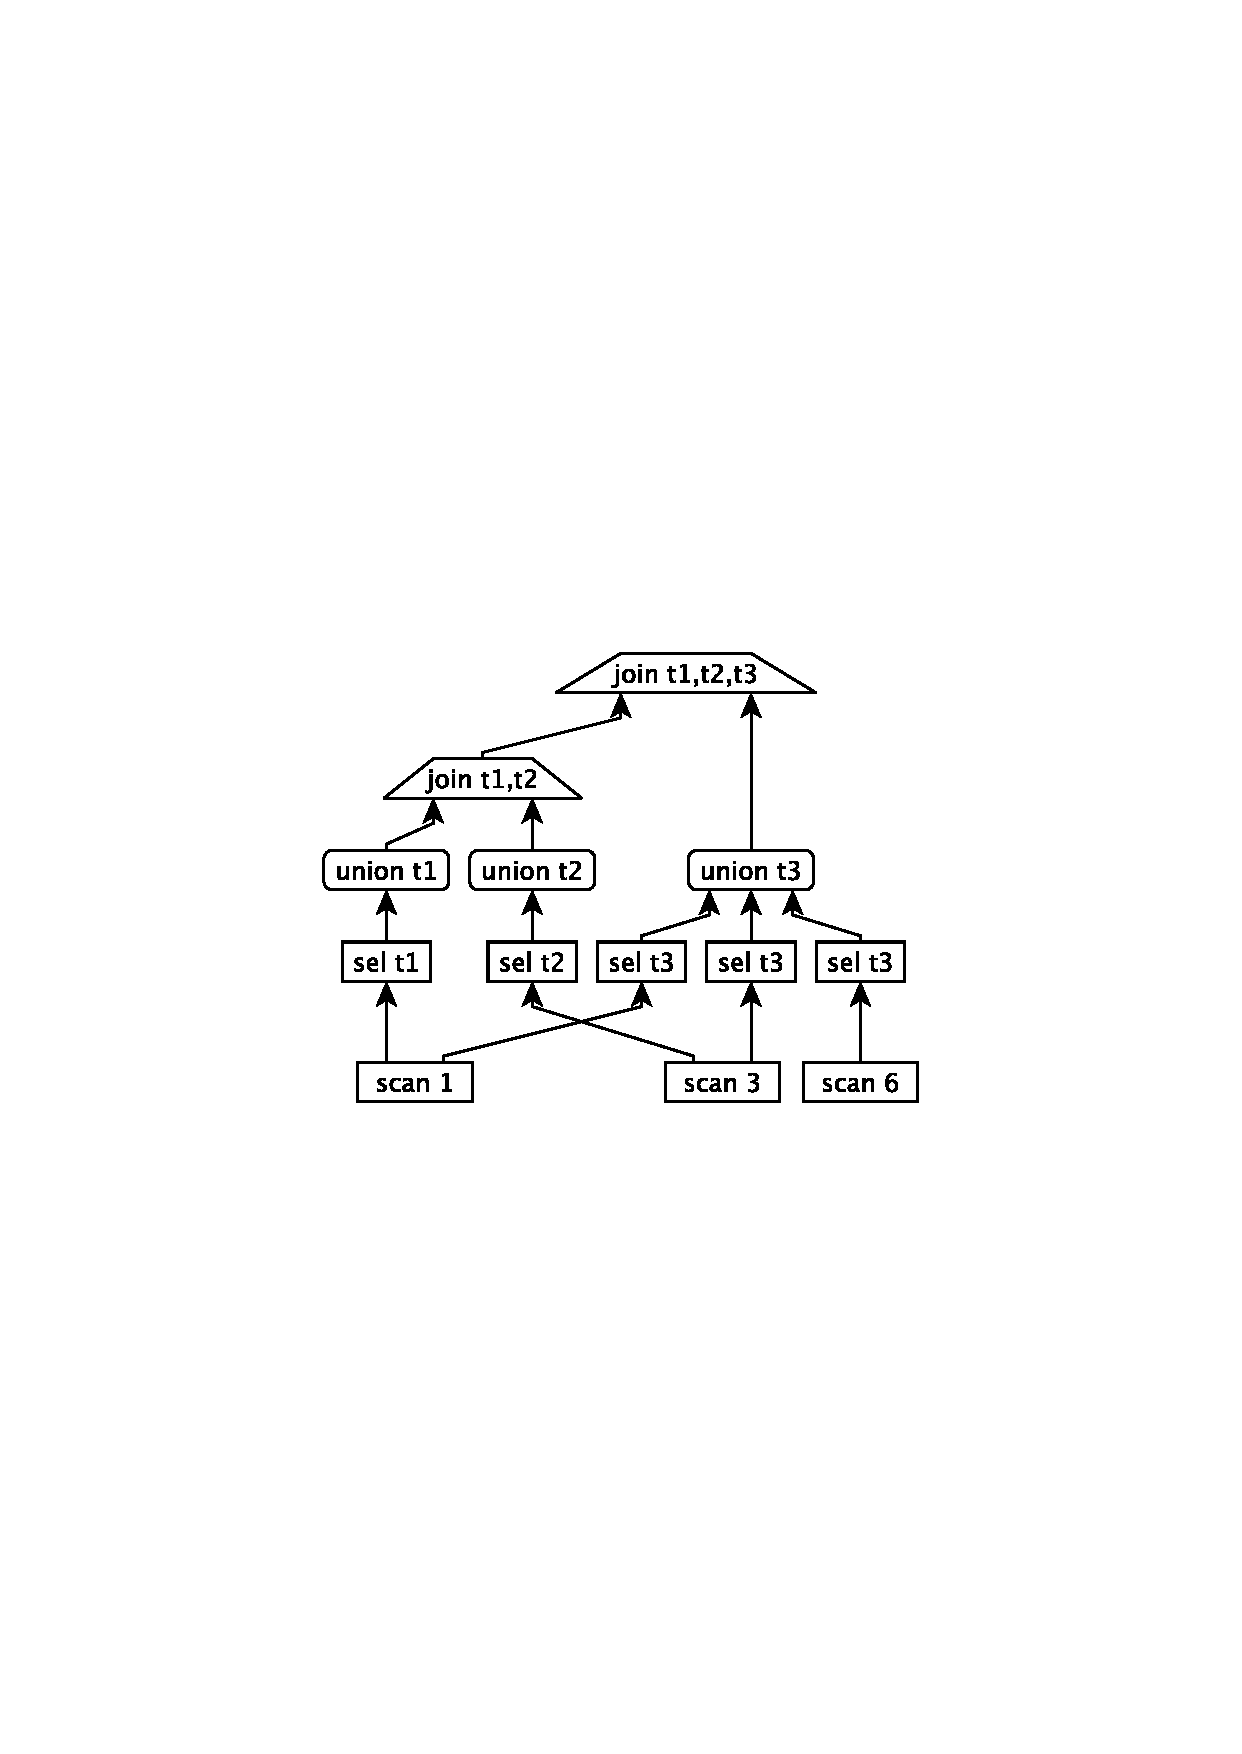
\includegraphics[width=0.6\linewidth]{figs/plan.pdf}
  \caption{Query plan for a query with three triple patterns and two
    sources.}
\label{fig:plan}
\end{figure}

\begin{example}
  Fig.~\ref{fig:plan} shows an example query plan for a query
  consisting of three triple patterns $t_1,t_2,t_3$ and two 
  sources $s_1,s_2$. There are six source scan operators $s_1^{t_1},
  s_2^{t_1}, s_1^{t_2}, \ldots$ for all combinations of triple
  patterns and sources. The source scan operators also have a rank,
  determining their processing order (here $s_2^{t_1}$ is processed
  first). The output of the unions for each triple pattern are joined
  using two symmetric hash joins. \dtr{Fig. not clear}
\end{example}


\subsection{Pareto Optimal Plans} 
Optimality is not clearly defined in the Linked Data context. Traditionally, completeness is assumed such that all results have to be computed. Optimality in this case is defined with respect to processing cost, and optimization techniques aim to find plans that are cost-optimal, i.e. produce all results at lowest costs. As discussed, completeness is not practical in Linked Data query processing and existing approaches (select and) process only a few sources~\cite{harth_data_2010,ladwig_linked_2010}. Not only cost but also the number of results have to be considered here. Further, other criteria such as the trustworthy of sources and the quality of data may play an important role. This results in a \emph{multi-objective} optimization problem. 

For a query $Q$, % = \{t_1, \ldots, t_n\}
the goal is to compute the skyline (Pareto set) of query plans that represent different trade-offs between multiple objectives. For clarity of presentation, we will focus on the two main objectives of maximizing \emph{output cardinality}, $card(\cdot)$, and \emph{processing cost} $cost(\cdot)$. Further, we define cost as $score(\cdot) = \frac{1}{cost(\cdot)}$ such that the objective is to maximize the score and output cardinality.  \todo{use cost instead of score everywhere}
The skyline of a set of solutions is defined using a \emph{dominance}
relation that relates the multiple objectives. A query plan is considered to dominate another plan, if it is at least as good in all objectives and better in at least one objective:

\begin{definition}[Dominance]
  Given two query plans $p_1,p_2$, $p_1 \mbox{ \textnormal{dominates}
  } p_2$ ($p_1 > p_2$) if both, score and cardinality, of $p_1$ are greater or equal
  to the score and cardinalty of $p_2$ and either score or
  cardinality is strictly greater than the score or cardinality of
  $p_2$, i.e. $score(p_1) \geq score(p_2) \wedge card(p_1) \geq
  card(p_2) \wedge ((score(p_1) > score(p_2) \vee card(p_1) >
  card(p_2)) \Rightarrow p_1 > p_2$.
\end{definition}


\begin{definition}[Pareto Optimal Plans]
  Given an query $Q$ and a set of query plans $P(Q)$, the \emph{Pareto}
  set $P^*(Q) \subseteq P(Q)$ comprises all plans that are not
  dominated by any other plan in $P(Q)$, i.e. $P^*(Q) = \{p_i \in P(Q) | \neg\exists p_j\in P(Q), p_j  > p_i\}$. We denote the set of
  dominated plans as $P^-(Q) = P(Q) \setminus P^*(Q)$. The set of \emph{optimal plans} for a query $Q$, denoted as $P^+(Q)$, is the Pareto set of plans for $Q$, i.e. $P^+(Q) = P^*(Q)$.
\end{definition}


\section{Dynamic Programming Based Optimization}
\label{sec:opt}
In this section we propose how to adopt the dynamic
programming (DP) solution~\cite{selinger_access_1979} to the 
multi-objective Linked Data query optimization problem. 

DP for query optimization works in a
bottom-up fashion, constructing the query plan starting from the
leaves, which are scan operators to access
relations. DP is is used to deal with the
exponentially large search space of possible query plans. It takes
advantage of the \emph{optimal substructure} of the query optimization
problem, i.e., the optimal query plan can be constructed from
optimal subplans. Non-optimal subplans can be
discarded during the process to reduce the search space.


Applied to Linked Data query processing, we propose to construct access plans $P(t)$ for every triple patterns $t \in Q$. These \emph{atomic plans} are then successively combined 
%using join operators 
to create \emph{composite plans} for larger subexpressions $T \subseteq Q$. 
For instance, to construct a query plan for the expression $T=t_1\Join t_2$, the optimizer may consider all possible pairs $\{(p1,p_2), p_1 \in P(t_1),p_2 \in P(t_2)\}$ as possible combination of plans. When combining two plans $p_1,p_2$ to form a new plan $p$, we
write $p = \mathtt{cmb}(p_1,p_2)$. At each stage, the optimizer 
try to reduce candidates subplans by discarding those that cannot be part of an optimal solution. That is, before constructing plans for larger subexpressions the optimizer creates $P^+(T) \subseteq
P(T)$, the set of optimal plans for every subexpression $T$. 
%In the case of Linked Data
%query processing, the optimality of a plan is determined according to
%multiple objectives. 

%, i.e., the set of optimal plans is the set of
%Pareto-optimal plans, $P^+(T) = P^*(T)$.

In the following, we firstly discuss how to estimate the optimality of atomic plans as well as composite plans for any expressions $T \subseteq Q$. Then we discuss the main problems that arise when applying the DP solution to this problem of multi-objective Linked Data query optimization.  Because query plans are no longer required to produce all results, we will
discuss a relaxation of the comparability constraint. Then, we study the effect of operator sharing on query optimization and introduce upper and lower bounds on plan
costs. Finally, we prove that the multi-objective query optimization problem still has optimal
substructure and that the dynamic programming solution constructs the
optimal solution, i.e. the skyline of query plans.

\subsection{Estimating Cost and Cardinality of Plans}
\label{sec:estimation}
For the presented structure of a Linked Data query plan and its operators, many existing techniques can be used to systematically estimate cost \cite{stocker_sparql_2008,neumann_scalable_2009,huang_selectivity_2010}. An essential factor for cost estimation is cardinality. While not only input cardinality but also output cardinality may be used for estimating the cost of some operators, optimizing based on cost alone does not guarantee that the resulting plans are also optimal with respect to output cardinality. 
%Instead of cardinality, the work discussed here is also applicable to other 
%In fact, not 
%%Further, other optimization objectives such as 
%only cost and cardinality but other objectives such as quality and relevance, which may have even smaller overlap with cost, have 
%Thus, estimating the optimality of a plan requires 
%For certain operators, input cardinality is not the same as 

%In this case, not only the cost but also the output cardinality are associated with query operators. 
We will now discuss straightforward estimates that will be needed in this work (and refer the readers to more specific work on cost and join size estimations for more advanced techniques \cite{stocker_sparql_2008,neumann_scalable_2009,huang_selectivity_2010}):

\textbf{Operators.} The output cardinality of the source scan operator is the same as the size of the source, i.e. $card(scan_d) = |T^d|$. 
% If the source is not locally available, it will be
%retrieved remotely. 
%A Linked Data source may contain arbitrary
%data and may therefore contain inputs for other triple
%patterns. If the source scan is an input for more than one operator,
%the data will only be retrieved once and will then either be kept in a
%local buffer for subsequent scans or, in the case of push-based
%execution, immediately be pushed to all subsequent operators.
This source size statistics can be directly obtained from the source index discussed before. 
For union, cardinality is the sum of the cardinalities of its inputs: $card(\cup(I_1,...,I_n)) = \sum_{i=1}^n card(I_i)$. 
The cardinality for selection and join depends on selectivity estimates $sel(\cdot)$, i.e. $card(\sigma_t(T_d)) = sel(t) \times |T_d|$ and $card(t_i \Join t_j) =
sel(t_i \Join t_j) \times card(t_i) \times card(t_j)$, respectively. 
%\textbf{Join.} The output cardinality of a join between triples obtained for the two patterns $t_i,t_j$ is given by its selectivity: 
Costs for scan, selection, union and join are $cost(scan_d) = h_s \times |T^d|$, $cost(\sigma_t(T_d))=h_\sigma \times |T_d|$, $cost(\cup) =
h_\cup \times card(\cup)$, $cost(\Join) =
h_\Join \times card(\Join)$. Thus, cost is assumed to be proportional to cardinality but different weights $h_s,h_\sigma,h_\cup,h_\Join$ are used for different operators. The weight factor $h_\Join$ for instance, depends on the
join algorithm employed. As in previous work on Linked Data query processing, we use symmetric hash join~\cite{ladwig_linked_2010,sihjoin_2011}. In case of operator sharing, separate cost
models for the first source scan (when the data is retrieved over the
network) and subsequent scans (when the data has already been
retrieved) are used. We use $cost_2(scan_d) = (1 - b) \times cost_1(scan_d)$, where $cost_1$ denotes first time cost, $cost_2$ stands for cost for each subsequent scan, and $b$
is a parameter to control the benefit achievable through operator sharing.


\textbf{Atomic Plan.} The cardinality of an access plan $p(t)$ is captured by its root node, i.e. $card(p(t)) = card(\cup_t)$. Its cost is calculated as the sum of the cost of its nodes. Source scan operators are marked after first time usage so that the right cost model can be determined for this calculation. 

\textbf{Composite Plan.} Composite plans capture the joins between results obtained for several triple patterns (outputs of access plans). Thus, for an expression $T = t_i\Join t_j$, $card(p(T))  = card(t_i\Join t_j)$ and $cost(p(T))  = cost(t_i\Join t_j)$.


\subsection{Comparability}
\label{sec:comparability}
% The dynamic programming algorithm works in a bottom-up fashion,
% constructing the query plan starting from the leaves, which in the
% classic problem are scan operators to access relations. Dynamic
% programming is used to deal with the exponentially large search space
% of possible query plans. It takes advantage of the optimal
% substructure of the classic query optimization problem, i.e., the
% optimal query plan can be constructed from optimal sub-plans. This
% enables the optimizer to prune non-optimal plans at each stage and
% only retain optimal sub-plans, reducing the search space
% significantly.

Pruning suboptimal plans is an essential part of the dynamic programming solution to
query optimization. 
%However, the optimizer must take care not to
%discard plans that may be part of an overall optimal solution, which
%then would no longer be found. 
For this, the notion of \emph{comparability} was introduced, which is an equivalence relation $\sim$ over plans. It determines which plans are comparable, based on which  
% according
%to some pre-defined properties. 
the optimizer can decide which plans are suboptimal. The optimizer can prune all but the optimal plans for each of the equivalence classes that are induced by $\sim$. 

In the traditional setting, atomic operators and plans comprising them are \emph{comparable when they produce the same output}. This comparability relation is applicable because input relations are determined by the query such that operators used to process them produce the same output and vary only with regard to cost. The optimizer than chooses how to process data (e.g. table or index
scan) based on cost estimates. In Linked Data query processing, however, the selection of
sources (represented by source scan operators) is part of query
optimization. Thus, the optimizer decides both \emph{what and how data shall be processed}. 
If we apply the comparability concept as defined
previously, each unique combination of source scan operators may yield different results and thus, would be represented by a separate equivalence class of query plans. Given there
are potentially hundreds of Linked Data sources for a single query, this may result in a search space where query optimization is no longer affordable.

However, we note that given the objectives here are cardinality and cost, we are not interested in which results but how many results will be produced. 
%is no longer required, 
Accordingly, a relaxation of this comparability relation can be employed that enables the optimizer to prune plans
more aggressively.

\begin{definition}
  \label{def:comparability}
  Two query plans $p_i, p_j$ are \emph{comparable} if they produce results for the same expression, i.e. $p_i(T_i) \sim  p_j(T_j)$ if $T_i = T_j$. 
\end{definition}

This relaxation means that comparable plans produce the same type of results (bindings for the same pattern), but may vary in the number as well as the actual results produced (different bindings). 

Besides results, other aspects have been incorporated into the comparability relation. For instance, plans may be considered comparable when they produce same results (same type of results), and these results are ordered \dtr{cite}. 
%when considering orders: a non-optimal sub-plan might produce ordered output, which can
%be efficiently used by sort-merge joins later in the query plan and
%should therefore not be discarded at the first possibility.
%Considering other properties such as interesting orders, is of course
%possible, but 
Besides this aspect of interesting orders, the inclusion of other objectives such as relevance and quality would also require a different notion of comparability.  
%For clarity, we omit additional constraints that may be added to. 

\subsection{Monotonicity}
\label{sec:sharing}
% As discussed, the query optimization algorithm based on dynamic
% programming constructs optimal plans for a given query $Q$ by starting
% with plans for single triple patterns $t \in Q$ and successively
% combining plans $P(T_1), P(T_2)$ for subexpressions $T_1,T_2 \subset
% Q, T_1 \cap T_2 = \emptyset$ to create plans $P(T)$ for subexpressions
% $T = T_1 \cup T_2$. In order to minimize the search space when
% creating plans $P(T)$, we prune plans from $P(T_1), P(T_2)$ that
% cannot be part of an optimal plan for $T$.

% In query optimization for relational databases, a plan is usually
% considered to be optimal if it has the lowest cost. Therefore it is
% possible to prune all but one plan for each equivalence class (as
% defined in the previous section) to obtain the set of optimal plans
% $P^*(T)$ for a given expression $T$. For optimization of Linked Data
% queries, however, there are two reasons why this is not as simple: 1)
% we no longer use a single dimension (such as cost) to assess query
% plans, but multiple dimensions (cost and cardinality) and 2) we employ
% operator sharing, which means that the cost function is no longer
% monotonic with regard to combining query plans. We tackle the problem
% of constructing Pareto-optimal query plans in the next section. Here,
% we consider each dimension separately and examine the effect of
% operator sharing on query optimization using dynamic programming.

A central requirement for the DP solution here is that the scoring function must be \emph{monotonic} with respect to plan combination. 
%Without this, the problem no longer has optimal substructure \todo{find something we
%  can cite for this}. 
Only then, subplans can be pruned because it can be guaranteed that they cannot be part of optimal plans. Here, plans have to be compared with respect to different objectives. We will now discuss the monotonicity of the functions employed for cost and cardinality. 
%Given monotonic functions for every 
%This still holds in the context of

\textbf{Cardinality.} Atomic plans are combined to capture joins between results. The monotonicity of the cardinality function can be established because the cardinality function for join is monotonic:

\begin{lemma}
  Given a query $Q$, let $T,T' \subset Q$ be two subexpressions of
  $Q$, such that $T \cap T' = \emptyset$. Let $p_1,p_2 \in P(T)$ and
  $p' \in P(T')$ be plans for $T$ and $T'$. Then we have $card(p_1) \leq
  card(p_2) \Rightarrow card(\mathtt{cmb}(p_1,p')) \leq
  card(\mathtt{cmb}(p_2,p'))$.
\end{lemma}
\begin{proof}
  % The output cardinality of combined plan is determined by the input
  % cardinality (i.e., the output cardinality of the two combined plans)
  % and the selectivity of the join operator used to combined the two
  % plans.
  The plan combinations above capture the expression $T \Join T'$. According to the function $card(T \Join T')$, we can write the condition in
  the theorem as $card(p_1) \leq card(p_2) \Rightarrow card(p_1)
  \times card(p') \times sel(T \Join T') \leq card(p_2) \times card(p') \times
  sel(T \Join T')$. This is true due to monotonicity of multiplication.
\end{proof}

\textbf{Cost.} For cost estimation, operator sharing is taken into
account. Because the costs of first and subsequent scans vary, the
cost of the source scan operator changes when a plan is combined with
another plan that shares that operator.
%Monotonicity is not clear which may cause
%the optimizer to miss the overall optimal plan.
Suppose we have two plans $p,p'$ for the subexpression $T \subset Q$
and a plan $p_t$ for a triple pattern $t$ such that $Q = T \cup
\{t\}$, and $cost(p) > cost(p')$. The optimizer would consider $p'$ to
be the optimal plan for $T$ and discard $p$ to form
$P^+(T)=\{p'\}$. Now, because of operator sharing it is possible that
the cost of the combination of two plans is less than the sum of the
cost of the two combined plans, i.e. it is possible that
$cost(\mathtt{cmb}(p,p_t)) < cost(\mathtt{cmb}(p',p_t))$ if $p$ and
$p_t$ share the same source such that the cost of $p_t$ when combined
with $p$ is much lower than the cost of $p_t$ that is combined with
$p'$. In this case, $p'$ should not be part of $P^+(T)$.

% To avoid this problem, We need to make sure that the cost and
% cardinality functions are \emph{monotonic} with regard to plan
% combination, meaning that the following conditions must hold:
% \[ cost(p_1) \leq cost(p_2) \Rightarrow cost(\mathtt{cmb}(p_1,p'))
% \leq cost(\mathtt{cmb}(p_2,p')) \]
% \[card(p_1) \leq card(p_2) \Rightarrow card(\mathtt{cmb}(p_1,p'))
% \leq card(\mathtt{cmb}(p_2,p'))\]
% \todo{should we add a proof that the monotonicity of the card function
%   is not violated when employing operator sharing?}

\textbf{Cost Bounds for Partial Plans.} In order to take this effect
of operator sharing into account when calculating the cost of a
partial plan $p$, we define upper and lower bounds for $p$ based on
larger plans that use $p$ as subplans:

\begin{definition}[Lower and Upper Bound Cost]
  \label{def:bounds}
  Given a query $Q$, the subexpressions $T \subset Q$, $T' = Q
  \setminus T$, a plan $p \in P(T)$, and let $P^p(Q) \subseteq P(Q)$
  be the set of all plans for $Q$ that are constructed as combinations
  of $p$ and plans in $P(T')$: $P^p(Q) = \{\mathtt{cmb}(p,p') | p' \in
  P(T')\}$.  Then, we have \emph{lower bound cost} for $p$ as
  $cost_L^Q(p)= MAX\{cost(p)| p \in P^p(Q)\}$ and \emph{upper bound
    cost} for $p$ as $cost_L^Q(p)= MIN\{cost(p)| p \in P^p(Q)\}$.
\end{definition}

Intuitively, a plan $p_i$ for a subexpression $T$ of $Q$ is ``worse''
in terms of cost than another plan $p_j$ for $T$, if all plans for $Q$
that are based on $p_i$ have higher cost than all plans for $Q$ that
are based on $p_j$, i.e., if $cost_L^Q(p_i) > cost_U^Q(p_j)$. Based on
these bounds, we can establish the monotonicity of plan cost with
respect to plan combination as follows:
  
\begin{lemma}
  Let $T,T' \subset Q$ be two subexpressions of $Q$ such that $T \cap
  T' = \emptyset$ and $p_1,p_2 \in P(T)$ and $p' \in P(T')$ be plans
  for $T$ and $T'$, respectively. We have
    \[ cost^Q_U(p_1) \leq cost^Q_L(p_2) \Rightarrow
    cost^Q_U(\mathtt{cmb}(p_1,p')) \leq
    cost^Q_L(\mathtt{cmb}(p_2,p')) \]
\end{lemma}
\begin{proof}
  This follows directly from the definition of $cost^Q_L$ and
  $cost^Q_U$ in Def.~\ref{def:bounds}. Any plan for $Q$ that is
  constructed as a combination of $p'_1 = \mathtt{cmb}(p_1,p')$, i.e.,
  any plan in $P^{p'_1}(Q)$, is also a combination of $p_1$ (because
  $p'_1$ is a combination of $p_1$). From this follows that
  $P^{p'_1}(Q) \subseteq P^{p_1}(Q)$ and $cost^Q_U(p'_1) \leq
  cost^Q_U(p_1)$. For $p_2$ and $p'_2 = \mathtt{cmb}(p_2,p')$ we get
  in the same way that $cost^Q_L(p'_2) \geq cost^Q_L(p_2)$. With this
  we see that $cost^Q_U(p_1) \leq cost^Q_L(p_2) \Rightarrow
  cost^Q_U(p'_1) \leq cost^Q_L(p'_2)$, meaning the lemma is true.
\end{proof}

Based on these results for cardinality and cost monotonicity, we now
refine the dominance relation to make it applicable to subplans,
i.e. plans for strict subexpressions of $Q$:

\begin{theorem}
  \label{def:dominates_bound}
  Given a query $Q$, a subexpression $T \subset Q$ and two plans
  $p_1,p_2$ for $T$, $p_1 > p_2$ if
  $card(p_1) \geq card(p_1) \wedge cost_U^Q(p_1) \leq cost_T^Q(p_2)
  \wedge (card(p_1) > card(p_2) \vee cost_U^Q(p_1) < cost_T^Q(p_2))$.
\end{theorem}

This is the main result needed for pruning. A subplan is suboptimal and thus can be pruned if it is dominated in the sense specified above. 

% With the lower and upper bounds we can reestablish the monotonicity of
% plan costs, however in a less restrictive form:

% \begin{theorem}
%   Given two plans $p_1,p_2$ for a subexpression $T$ and a plan $p'$
%   for a subexpression $T'$, such that $T \cap T' = \emptyset$, the
%   following condition holds:
%   \[ cost_U^{T\cup T'}(p_1) \leq cost_L^{T\cup T'}(p_2) \Rightarrow 
%   cost(\mathtt{cmb}(p_1,p') \leq cost(\mathtt{cmb}(p_2,p')) \]
% \end{theorem}
% \begin{proof}
%   \todo{proof}
% \end{proof}

\textbf{Cost Bound Estimation.} In the form of
Definition~\ref{def:bounds}, the calculation of the lower and upper
bounds of a plan $p$ requires constructing all plans based on
$p$. This is of course very cost intensive and defeats the purpose of
pruning. We therefore try to estimate the bounds by determining the
maximal possible benefit that is achievable through operator sharing
for a particular plan. 

As the source scan operator is the only shareable operator, we can
calculate the maximal possible benefit for a particular plan $p$ by
using the source index to retrieve all sources for triple patterns not
covered by $p$ and aggregating the benefit for all sources that are
also used by $p$.

We only use the maximal benefit when comparing two plans $p,o$ to decide
whether one plan dominates the other. In this case, we can obtain more
a more precise benefit $p$ by only aggregating the benefit for sources
that are not part of $o$. We therefore define the maximal benefit of a
plan $p \in P(T)$ in terms of another plan $o \in P(T)$:

\begin{definition}
  Given a query $Q$, a source index $I$, and two query plans $p,o \in
  P(T), T \subset Q$, let $S_p,S_o$ be the sets of sources retrieved
  by source scan operators in $p,o$, respectively. The maximal benefit
  of $p$ w.r.t $o$ defined as $m_o(p) = \sum_{t \in Q \setminus T}
  \sum_{(d,r_d) \in I(t), d \notin S_p \cap S_o } b \cdot
  cost_1(scan_d)$, where $b$ is the sharing benefit and
  $cost_1(scan_d)$ is the cost for the first read of the source scan
  operator for source $d$, as introduced in Sec.~\ref{sec:ops}.
\end{definition}

With the maximal benefit, we again define a more strict dominance
relation $>_b$ using the maximal benefit:

\begin{theorem}
  Given a query $Q$, a subexpression $T \subset Q$ and two plans
  $p_1,p_2 \in P(T)$, then $p_1 \mbox{\textnormal{ strictly dominates
    }} p_2$ ($p_1 >_b p_2$) if $card(p_1) \geq card(p_1) \wedge
  cost(p_1) \leq cost(p_2) - m_{p_1}(p_2) \wedge (card(p_1) >
  card(p_2) \vee cost(p_1) < cost(p_2) - m_{p_1}(p_2))$.

  Whenever $p_1$ strictly dominates $p_2$ then $p_1$ dominates $p_2$:
  $p_1 >_b p_2 \Rightarrow p_1 > p_2$.
\end{theorem}
\begin{proof}
  
\end{proof}

With this theorem we can use the maximal benefit to perform pruning
and be sure that no optimal plan is discarded.

\subsection{Pareto-optimality}
\label{sec:pareto}

The goal of the optimizer in the Linked Data query processing scenario
is to find the overall skyline (or Pareto set) of query plans, while
pruning as many plans as possible at each step. We will show that we
can retain only non-dominated plans for each subexpression and still
find the complete overall skyline, i.e., we show that the optimization
problem still has optimal substructure.

The goal is to find the optimal solution for query $Q$, in this case
the optimal solution is the set of Pareto-optimal query plans $P^+(Q)
= P^*(Q)$. To prove that the problem has optimal substructure, we need
to show that we can construct $P^*(Q)$ by splitting $Q$ into
subproblems $T \subset Q$ and then combining optimal solutions
$P^*(T)$ for the subproblems. In particular, this means that a
non-optimal solution for a subproblem must not be part of an optimal
solution for a superproblem.

% The smallest subproblem is a singleton subset of $Q$, i.e., a single
% triple pattern $t$. An optimal solution for this problem is a set of
% Pareto-optimal plans $P^*(\{t\})$. Each such plan $p_t$ is an access
% plan, consisting of a set of source scan operators, whose output is
% fed into separate selection operators and then into a single union
% operator.

% The first step where solutions for subproblems are combined is
% constructing query plans for 2-element subsets of $Q$, i.e., joins
% between base inputs. We show that we can construct $P^*(\{t_1,t_2\})$
% by combining optimal solutions for $t_1$ and $t_2$, i.e.,
% $P^*(\{t_1\})$ and $P^*(\{t_2\})$, for all $t_1,t_2 \in Q$ with $t_1
% \neq t_2$. Let $S$ be the set of all plans constructed by combining
% Pareto-optimal plans for $t_1$ and $t_2$: $S =\{\mathtt{cmb}(p_1,p_2)
% | p_1 \in P^*(t_1), p_2 \in P^*(t_2)\}$. Then we need to show that
% $P^*(\{t_1,t_2\}) = S^*$ or $P^*(\{t_1,t_2\}) \subseteq S$.

% \begin{align*}
%   P^*(\{t_1,t_2\}) \subseteq S &  \Leftrightarrow  \forall p^* \in
%   P^*(\{t_1,t_2\}) : p^* \in S \\
% &   \Leftrightarrow \forall p^* \in P^*(\{t_1,t_2\}) :
%   p^* = \mathtt{cmb}(p^*_1, p^*_2) \;\mathrm{with}\; p^*_1 \in
%   P^*(t_1), p^*_2 \in P^*(t_2)
% \end{align*}

% This means that all optimal, i.e., non-dominated, plans for $t_1,t_2$
% are a combination of non-dominated plans for $t_1$ and $t_2$,
% respectively.

% \todo{benutz kosten ohne bounds hier, oben dann beweisen dass wir beim
%   benutzen der bounds beim prunen irgendwas klappt}

\begin{theorem}
  Given a query $Q$ and two subexpressions $T_1,T_2 \subseteq Q$ with
  $T_1 \cap T_2 = \emptyset$, the set of optimal plans for $T_1 \cap
  T_2$ can be constructed from optimal plans for $T_1,T_2$, i.e.,
  $P^+(T_1 \cup T_2) = P^*(T_1 \cup T_2) \subseteq C =
  \{\mathtt{cmb}(p_1,p_2) | p_1 \in P^*(T_1), p_2 \in P^*(T_2)\}$.
\end{theorem}
\begin{proof}
  Let $p^* \in P^*(T_1 \cup T_2)$ be a plan that is a combination of a
  dominated plan for $T_1$ and a non-dominated plan for $T_2$, i.e.,
  $p^* = \mathtt{cmb}(p^-_1,p^*_2),p^-_1 \in P^-(T_1),p^*_2 \in
  P^*(T_2)$. This means that there is a non-dominated plan $p^*_1 \in
  P^*(T_1)$ that dominates $p^-_1$, but the combination of $p^*_1$
  with $p^*_2$ is dominated by the combination of $p^-_1$ and $p^*_2$:
  \[ \exists p^*_1 \in P^*(T_1) : \mathtt{cmb}(p^-_1,p^*_2) \text{
    dominates } \mathtt{cmb}(p^*_1,p^*_2)\] As $p^*_1$ dominates
  $p^-_1$ and $\mathtt{cmb}(p^-_1,p^*_2)$ dominates
  $\mathtt{cmb}(p^*_1,p^*_2)$, according to
  Def.~\ref{def:dominates_bound}, this implies (without loss of
  generality we assume that both objectives are strictly
  lesser/greater):
  \begin{eqnarray*}
    card(p^-_1) < card(p^*_1) &\wedge& card (\mathtt{cmb}(p^-_1,p^*_2)) > card(\mathtt{cmb}(p^*_1,p^*_2)) \\
    cost^Q_L(p^-_1) < cost^Q_U(p^*_1) &\wedge& cost^Q_U(\mathtt{cmb}(p^-_1,p^*_2)) > cost^Q_L(\mathtt{cmb}(p^*_1,p^*_2))\\
  \end{eqnarray*}
  However, with the montonicity of both, the cost and the cardinality,
  we have a contradiction, because $cost^Q_L(p^-_1) <
  cost^Q_U(p^+_1)$, but $cost^Q_U(\mathtt{cmb}(p^-_1,p^*_2)) >
  cost^Q_L(\mathtt{cmb}(p^*_1,p^*_2))$ (the same holds for the
  cardinality). With regard to our original proposition, this means
  that there is no plan $p^* \in P^*(T_1 \cup T_2)$, such that $p^*$
  is a combination of dominated plan $p^-_1$ and a non-dominated plan
  $p^*_2$. The same holds when $p^*$ is a combination of two dominated
  plans (we omit the proof for brevity). From this follows that all
  $p^* \in P^*(T_1 \cup T_2)$ are combinations of the non-dominated
  plans in $P^*(T_1)$ and $P^*(T_2)$ and therefore $P^*(T_1 \cup T_2)
  \subseteq C$.
\end{proof}

% Proof by contradiction: Suppose there is a non-dominated plan $p^* \in
% P^*(\{t_1,t_2\})$ that is a combination of a dominated plan for $t_1$ and
% a non-dominated plan for $p_2$:
% \[\exists p^* \in P^*(\{t_1,t_2\}) : p^* = \mathtt{cmb}(p^-_1,p^*_2),
% p^-_1 \in P^-(t_1), p^*_2 \in P^*(t_2) \] 

% This would mean that there is a non-dominated plan $p^*_1 \in
% P^*(t_1)$ that naturally dominates $p^-_1$, but the combination of
% $p^*_1$ with $p^*_2$ is dominated by the combination of $p^-_1$ and
% $p^*_2$:
% \[ \exists p^*_1 \in P^*(t_1) : \mathtt{cmb}(p^-_1,p^*_2)
% \text{ dominates } \mathtt{cmb}(p^*_1,p^*_2)\]

% This implies that the score and cardinality of
% $\mathtt{cmb}(p^-_1,p^*_2)$ are greater or equal than the score and
% cardinality of $\mathtt{cmb}(p^*_1,p^*_2)$, whereas the score and
% cardinality of $p^-_1$ is less than the score and cardinality of
% $p^*_1$ (because $p^*_1$ dominates $p^-_1$):

% \begin{eqnarray*}
%   score(p^-_1) < score(p^*_1) &\wedge& score(\mathtt{cmb}(p^-_1,p^*_2)) \geq score(\mathtt{cmb}(p^*_1,p^*_2))\\
%   card(p^-_1) < card(p^*_1) &\wedge& card (\mathtt{cmb}(p^-_1,p^*_2)) \geq card(\mathtt{cmb}(p^*_1,p^*_2)) \\
% \end{eqnarray*}

% However, we postulate that $card$ and $score$ are monotonic with
% regard to the combination of plans:
% \begin{eqnarray*}
%   score(p_1) \leq score(p'_1) &\Rightarrow& score(\mathtt{cmb}(p_1,p_2))
%   \leq score(\mathtt{cmb}(p'_1,p_2)) \\
%   card(p_1) \leq card(p'_1) &\Rightarrow& card(\mathtt{cmb}(p_1,p_2))
%   \leq card(\mathtt{cmb}(p'_1,p_2)) \\
% \end{eqnarray*}

% where $p_1,p'_1$ are any plans for the same expression and $p_2$ is a
% plan for a different, disjunct expression. 

% \todo{add bounds here}

% With the monotonicity of the $score$ and $card$ functions we have a
% contradiction, because $score(p^-_1) < score(p^*_1)$, but
% $score(\mathtt{cmb}(p^-_1,p^*_2)) \geq
% score(\mathtt{cmb}(p^*_1,p^*_2))$ (the same holds for the
% cardinality). With regard to our original proposition, this means that
% there is no plan $p^* \in P^*_{t_1,t_2}$ such that $p^*$ is a
% combination of a dominated plan $p^-_1$ and a non-dominated plan
% $p^*_2$. \todo{show that this also holds when both plans are
%   dominated} From this follows that all $p^* \in P^*_{t_1,t_2}$ are
% combinations of the non-dominated plans in $P^*_{t1}$ and $P^*_{t_2}$.


Although the relaxed comparability constraint allows the optimizer to
prune more aggressively than otherwise possible, we observe that the
goal of generating Pareto-optimal query plans again leads to a larger
search space.

\subsection{Optimizer Algorithm}

With the relaxed comparability constraint and the Pareto-optimality
in place, we can now present the query optimization algorithm for
constructing Pareto-optimal Linked Data query plans.

% \subsubsection{Pareto-optimal Access Plans for Triple Patterns}

% The first step in the dynamic programming algorithm for query
% optimization is creating Pareto-optimal access plans for single query
% triple patterns. As described in Section~\ref{sec:basicshape} these
% plans each consist of a set source scan operators whose output feeds
% into selection operators and then in a single union operator. Given a
% triple pattern $t$, we first use the source index to obtain the set of
% relevant sources $D = I(t)$.

% A naive solution to obtain the Pareto-optimal plans for $t$ would be
% to first create the set of all possible plans and then prune all
% dominated plans. However, we can construct a valid plan for $t$ from
% any subset of $D$, i.e., there is one possible plan for each element
% of the power set of $D$. As the size of the power set is $2^{|D|}$
% this is infeasible even for triple patterns that appear in only
% relatively few sources.

% \todo{add short description of the algorithm we use}

% \subsubsection{Pareto-optimal Dynamic Programming}

\begin{algorithm}
  \label{alg:plan}
  \DontPrintSemicolon

  \SetKwData{BestPlans}{bestPlans}\SetKwData{Null}{null}
  \SetKwFunction{Combine}{combine}

  \caption{\textsc{PlanGen}$(q)$}
  \KwIn{Query $q = \{t_1,\ldots,t_n\}$, Source index $I$}
  \KwOut{Pareto-optimal query plans \BestPlans{q}}

  \ForEach{$t \in q$}{
    $S \leftarrow \{ \cup(\{ \sigma_t(scan(d)) | d \in D \}) | D \in \mathcal{P}(I(t))\}$
%    $S \leftarrow \{\cup(C) | C \in \mathcal{P}(\{\sigma_t(scan(d)) | d \in I(t)\})\}$ \;
    \BestPlans{$\{t\}$}$\leftarrow \{p \in S| \nexists p' \in S : p'
    \mbox{ dominates } p \}$\;
  }

  \For{$i \leftarrow 2$ \KwTo $|q|$}{
    \ForEach{$T \subseteq q$ such that $|T| = i$}{
      \ForEach{$t \subset T$}{
        $S \leftarrow S \cup$ \Combine{\BestPlans{$\{t\}$},
          \BestPlans{$T \setminus \{t\}$}}\;
      }
      \BestPlans{$T$}$\leftarrow \{p \in S | \nexists p' \in S : p'
      \mbox{ dominates } p \}$\;
    }
  }
  \Return \BestPlans{q}
\end{algorithm}

\todo{show generation of access plans}

Algorithm~\ref{alg:plan} shows the method \textsc{PlanGen} that takes
a query $q=\{t_1,\ldots,t_n\}$ as input and returns the Pareto-optimal
plans to evaluate the query. During optimization, \textsf{bestPlans}
stores the best plans for all subsets of $q$. 

In the first step, the plans for single triple patterns are
created. For each triple pattern $t$ in $q$, first the relevant
sources are selected with help of the source index $I$. As we need to
consider all possible combinations of sources, we create the power set
$\mathcal{P}(I(t))$ of all sources. For each member $D$ of the power
set, we create an access plan, consisting of a selection and scan
operator $\sigma_t(scan(d))$ for each source $d \in D$ and a single
union operator $\cup$ that has the selection operators as input. $S$
then contains a set of access plans, one for each combination of
relevant sources. From this set, we then select only the
non-dominated, i.e., Pareto-optimal, access plans and store them in
\textsf{bestPlans}$(\{t\})$.

During the next iterations, joins between previously created plans are
calculated until all query triple patterns are covered. For iteration
$i$, we select all subsets $T \subset q$ with $|T|=i$. For each $t \in
T$ the algorithm creates all possible joins between the best, i.e.,
Pareto-optimal, plans for $t$ and $T\setminus \{t\}$. By selecting
only a single triple pattern from $T$ we create only left-deep plans,
but bushy plans would also be possible.  All these plans are stored in
$S$ and are comparable since they cover the same triple patterns
$T$. Finally, only the non-dominated plans from $S$ are selected and
stored in \textsf{bestPlans}$(T)$. After the last iteration,
\textsf{bestPlans}$(q)$ contains the Pareto-optimal left-deep plans
for $q$.

\todo{describe combine, duplicate source scan operators are combined
  here; description of cost calculation for such a DAG is in earlier
  section}


% \subsection{Adaptivity}
% The goal of adaptive query processing is to perform query optimization
% in the case were no complete knowledge is available and adapt the
% query processing at run-time by using newly available
% knowledge. During processing of Linked Data queries, new information
% about sources becomes available: 1) new sources may be discovered, 2)
% state accumulated inside join operators can be used to perform better
% estimates of join cardinalities for a particular source and 3) data
% properties may be observer to deviate from previous estimates.

% Here, we adopt techniques from previous research on adaptive query
% processing.

% \todo{what do we monitor? when is re-optimization done?}

% Linked Data query processing requires ranking to be performed not only
% at compile-time, but also continously at run-time in order to take
% advantage of knowledge gained during query processing. Using
% adaptive query processing techniques not only ranking can be
% performed, but full query optimization at run-time. 

% Weight distribution between cost and relevancy might change over time:
% at first, relevancy is more important, while later on, after results
% have been produced, cost becomes more important?


% \subsection{Implementation}
% \label{sec:impl}

% \todo{describe concrete implementation, in particular methods used for
% cost/result estimation and query strategies different from the optimal
% ones}

% \todo{dependencies between sources are not reflected by available
%   statistics, but indirectly captured using run-time reestimation of
%   result sizes using sampling etc.}



%%% Local Variables: 
%%% mode: latex
%%% TeX-master: "paper"
%%% End: 

%\input{section-processing}
\section{Related Work}
\label{sec:related}

\textbf{Linked Data Query Processing.} The concept of executing SPARQL
queries directly over Linked Data instead of a locally stored and
indexed copy was first introduced in \cite{hartig_executing_2009},
where link traversal is used to discover sources at runtime. In
\cite{harth_data_2010} a local source index based on QTrees is used to
speed up the discovery of relevant sources. Other previous work
\cite{ladwig_linked_2010,sihjoin_2011} proposes methods for ranking
sources at runtime according to their relevancy and a mixed execution
strategy that combines both, link traversal and source indexes, to
report results early. In this work we adopt the approach from
\cite{harth_data_2010} and employ a source index without any runtime
source discovery. %  along with the push-based Symmetric Hash Join
% operator from \cite{ladwig_linked_2010,sihjoin_2011}.


% \textbf{Dynamic Programming.}

% Faster enumeration of plans: \cite{moerkotte_analysis_2006,moerkotte_dynamic_2008}

% Iterative Dynamic Programming (approx): \cite{kossmann_iterative_2000}

\textbf{Multiobjective Query Optimization.} Multi-objective query
optimization was previously proposed in
\cite{papadimitriou_multiobjective_2001}, where it is discussed in the
context of Mariposa \cite{stonebraker_mariposa:_1996}, a wide-area
database system. The Mariposa optimizer splits the query tree into
subqueries and then obtains \emph{bids} from participating database
sites that specify a delay and cost for delivering the result of a
subquery. The goal of the optimzer is to obtain the Pareto optimal set
of plans with respect to cost and delay. While the authors do employ
dynamic programming to show that the Pareto set can be approximated in
polynomial time, it is not based on the classic dynamic programming
algorithm for query optimization proposed in
\cite{selinger_access_1979}. The problem is slightly different as
there is only a single query operation tree and for each operation
node the optimizer is provided a list of alternatives for implementing
the operation. In contrast, the classic dynamic programming
\cite{selinger_access_1979} does not consider only a single query tree
(and therefore a single order of operations), but builds and optimizes
physical query plans from the bottom up and considers all valid query
trees. In this work we extend the classic algorithm to support
multi-objective query optimization.

The approach presented in \cite{nie_joint_2001} optimizes query plans
not only for cost, but also for coverage (i.e. output cardinality) and
thereby integrates source selection into the query optimization
process. However, the optimization is performed by combining
(weighted) cost and coverage into a utility function that provides a
single measure to assess query plans. Using a single measure means
that traditional query optimization algorithms, such as dynamic
programming \cite{selinger_access_1979}, are directly
applicable. However, no true multi-objective optimization is
performed.


\textbf{Data Integration.}

Bucket algorithm: \cite{levy_querying_1996}

MiniCon algorithm: \cite{pottinger_minicon:_2001}

Optimization of cost and coverage (utility function):
\cite{nie_joint_2001}

Source selection: \cite{pomares_source_2010}

Query Planning in the Presence of Overlapping Sources:
\cite{bleiholder_query_2006}

survey materialized views: \cite{halevy_answering_2001}



%%% Local Variables: 
%%% mode: latex
%%% TeX-master: "paper"
%%% End: 

\begin{figure*}[htb]
  \vspace{-0.5cm}
  \centering
  \includegraphics[width=0.75\linewidth]{figs/all_queries.pdf}
  \includegraphics[width=0.24\linewidth]{figs/plans_skyline_by_m.pdf}
  \caption{a) Number of skyline and non-skyline plans for all queries
    and systems ($b=0.8, m=2000$), b) Skyline fraction for RD, RK for
    different value of $m$ ($b=0.8$).}
  \label{fig:queries}
  \vspace{-0.5cm}
\end{figure*}

\section{Evaluation}
\label{sec:eva}
Existing works in data integration~\cite{levy_querying_1996} and Linked Data query processing~\cite{harth_data_2010,ladwig_linked_2010} perform source ranking
without further optimization. We implement source ranking to select sources first, and then use the dynamic DP solution as proposed for Linked Data query optimization to optimize
the subsequent process. That is, the proposed query plan as well as
the operator sharing mechanism are employed to optimize cost. This is
to obtain a best-effort baseline, based on which we aim the study of
effect of the holistic treatment of source selection and query
processing, and the multi-objective optimization we propose. The
experiment shows that as opposed to our approach, the baseline yields
only a small fraction of the complete set of Pareto-optimal plans, and
the resulting suboptimal plans lead to much higher total cost when producing
the same number of results. 

%Compared to the baseline, resulting cost (measured in terms of total time needed for computing results) needed may be as 

%The evaluation of our approach consists of two parts. In the first, we
%evalute the benefit of using the dynamic programming query
%optimization algorithm for Linked Data query processing in a
%single-objective scenario. In the second part, we focus on the
%multi-objective optimization approach proposed in this paper.

% \subsection{Single-objective Optimization with Dynamic Programming}

% \subsubsection{Systems}


% \subsubsection{Results}



% \begin{figure}[htb]
%   \centering
%   \includegraphics[width=\linewidth]{figs/exec_queries.pdf}
%   \caption{Results for execution}
%   \label{fig:exec_queries}
% \end{figure}



\subsection{Systems}
\textbf{Our Approach.} We implemented three versions of our
approach. The first version (DP) implements all the proposed
techniques to produce the complete set of Pareto-optimal plans. The
second version (DPU) also uses operator sharing such that for
subsequent source accesses, the refined cost model applies. However,
the effect of this is not taken into account during pruning.  That is,
it uses directly the cost instead of the lower and upper bounds that
have been established to guarantee monotonicity of cost. Thus, at the
cost of compromising Pareto-optimality, DPU can prune more
aggressively and thus, is expected to exhibit better performance. This baseline can be seen as an approximate version of our approach that simply uses actual cost as an approximate estimate for bounds. 
%With
%this baseline, we aim to study the positive effect of using the
%proposed bounds on Pareto-optimality, and to find out whether the
%proposed technique for estimating the bounds is effective in reducing
%the overhead resulting from that. 
The third version (DPS) does not use
operator sharing at all, i.e. if a source is used for more than one
triple pattern it is retrieved multiple times. 
%We use DPS to study the effect the benefits operator sharing.
We use different settings for $b$ to study the effect of operator sharing. For example, with $b=0.8$ the optimizer assumes that 80\% of
the source scan cost is saved, i.e. subsequent reads cost only 20\% of the first read.

\textbf{Baselines.} Existing Linked Data approaches implement ad-hoc
source ranking to select few best
sources~\cite{harth_data_2010,ladwig_linked_2010}, and then process
these sources without further optimization. This processing represents
one single plan, whose optimality is unknown. We implement this source
ranking (RK) and a random source selection strategy (RD), and 
%Given the
%selected sources, 
apply our DP solution on top but only to
optimize the cost. 
% these baselines need to produce results from these
%sources. 
%In the same way proposed for our approach, this DP solution
%applies operator sharing so that sources can be reused. 
Instead of one
single cost-optimized plan, our approach however yields a Pareto-set
of query plans that represents different trade-offs between cost and
cardinality. Thus, we further extend these baselines to use different
combinations of sources that yield different plans.

Both baselines first retrieve all relevant sources $D$ for a query $Q$
from the source index, i.e. $D = \bigcup_{t \in Q} source(t)$. Then,
a set $\mathcal{D}$ containing $|D|$ different subsets of $D$, each
with size in the range $[1,|D|]$ is created.
%The number of  captured by and $|\mathcal{D}| = |D|$. 
The baselines differ in how these
subsets are selected:
\begin{itemize}
\item Baseline RD randomly selects the $|D|$ subsets.
\item Baseline RK first ranks sources in $D$ by the number of
  contained triples that match query triple patterns, calculated as
  $score(d) = \sum_{t \in q} card_d(t)$. The subsets are created
  by starting with the highest ranked source and then successively
  adding sources in the order of their rank to obtain $|D|$ subsets in
  total.
\end{itemize}
Each element in $\mathcal{D}$ represents a combination of sources, for each of which a query plan is created. As a
result, we have a set of plans, which vary in the number of results as
well as cost because different combinations of sources are used.
% using a standard dynamic
%programming optimizer (i.e., no multi-objective optimization). Sharing
%of source scan operators is also employed where possible.

Note that our approach not only selects sources (source scan
operators) but also for which triple patterns these sources are used
(selection operators), while the sources selected for the baselines
are used for all triple patterns. In order to obtain even more plans
that further vary in the number of results they produce, we create an
additional set of $m$ plans for each previously created plan of the
baselines RK and RD by
randomly removing a subset of the inputs (selection operators) from
the unions at the root of their access plans.
%In particular, to create a new plan from an
%existing plan, for each union that is root of an access plan, we
%remove a random subset of its input (selection) operators. 
%If the source scan operator that is input for a removed selection operator is
%not shared it is also remove from the plan.
%Any invalid plans that are constructed in this way (e.g., all inputs of an union might have been) are discarded. 
In the end, each baseline has at most $m \cdot |D|$ plans that vary
in terms of results (of which only $|D|$ plans actually vary in cost).

%These baselines optimize source selection independent from the
%subsequent computation of results. While the goal of source selection
%is to choose those that contribute many results, the subsequent
%optimization focuses on cost. Compared to them, our approach not only
%jointly optimize sources section and result computation but also,
%considers cardinality and cost at the same time. Our goal is to study
%the effect of this joint optimization on the Pareto-optimality of
%plans. Further, we will investigate the effect of using non-optimal
%plans on the result....
%While this effect is expected to be positive, the increased complexity of the planning problem also leads to additional cost. Thus, we will also investigate whether this overhead can be justified by looking at the total processing time needed for producing several fixed fraction of results.  

%
%\textbf{Parameters.} Parameter $b$ specifies the benefit that is
%assumed during query planning for sharing of source scan
%operators. For example, with $b=0.8$ the planners assume that 80\% of
%the source scan cost is saved, i.e., second and subsequent reads of a
%source scan operator cost only 20\% of the first read.
%
%For RD and RK, parameter $m$ describes the number of additional plans
%that were generated by randomly remove selection and source scan
%operators.

\begin{figure}[htb]
  \vspace{-0.1cm}
  \centering
  \includegraphics[width=0.48\linewidth]{figs/plans_q2_all.pdf}
  \includegraphics[width=0.48\linewidth]{figs/plans_q2_sky.pdf}
  \caption{Plans for query Q1 on all systems: a) all plans and b)
    skyline plans ($b=0.8,m=2000$).}
  \label{fig:pareto_q2_skyline}
  \vspace{-0.5cm}
\end{figure}

\subsection{Setting} As data, we use real-world Linked Data currently available on the Web. We generate queries and process them against Linked Data sources on the Web to obtain a total of 1,909,109 triples from various popular datasets such as DBpedia, Freebase, New York Times, GeoNames and LinkedMDB. The number of Linked Data sources from which all data were retrieved is 516,293. During this process, we observed that network latency greatly varies. In order to systematically study the effects of query processing, we thus decided to download these data, and to simulate Linked Data query processing on one single machine. To reflect network cost, we tried different settings, including the average of 1.5s that we could observed on real-world sources. Performance differences between systems were however not sensitive to these settings. 

As queries, we focus on 14 BGP queries that have non-empty results. The result size is in the range from 1 to 836. We use queries that largely differ in the number of results to discuss the effect of Pareto-optimality on the cost-cardinality trade-off in detail. These queries belong to different classes of complexity, which is reflected in the number of triple patterns. For the classes of 3, 4 and 5 patterns, we have 4, 5, and 5 queries, respectively. 


%Table~\ref{tab:queries} shows various
%statistics for all evaluation queries.

%This dataset was then
%indexed in a source index and used for the evaluation. 
%As the source index contained too many sources for the multi-objective
%optimization approach to deal with, we randomly aggregated sources
%during the creation of access plans into a set of $k=5$ virtual
%sources. The size of the virtual sources follows a Zipf distribution
%with exponent $2$.


%
%\begin{table}[htb]
%  \centering
%  \begin{tabular}{l|c|c|r}
%    Query & \#Pat. & Shared [kT] & \#Res. \\%& Join-Sel. SD \\ 
%    \hline
%
%    Q2  & 3 & 1,393 & 24  \\%& 3.26\textsc{e}-5 \\
%    Q5  & 3 & 1,425 & 13  \\%& 4.95\textsc{e}-5 \\
%    Q15 & 3 & 1,401 & 11  \\%& 2.59\textsc{e}-5 \\
%    Q19 & 3 & 1,434 & 836 \\%& 4.36\textsc{e}-5 \\
%    \hline
%    Q1  & 4 & 1,426 & 2   \\%& 1.30\textsc{e}-3 \\
%    Q3  & 4 & 1,892 & 3   \\%& 1.89\textsc{e}-5 \\
%    Q4  & 4 & 1,415 & 60  \\%& 9.58\textsc{e}-3 \\
%    Q6  & 4 & 2,081 & 6   \\%& 2.62\textsc{e}-3 \\
%    Q7  & 4 & 1,369 & 106 \\%& 2.75\textsc{e}-3 \\
%    \hline
%    Q9  & 5 & 1,405 & 17  \\%& 5.26\textsc{e}-3 \\
%    Q14 & 5 & 1,830 & 20  \\%& 3.71\textsc{e}-3 \\
%    Q16 & 5 & 2,396 & 1   \\%& 2.10\textsc{e}-3 \\
%    Q17 & 5 & 1,409 & 1   \\%& 8.92\textsc{e}-3 \\
%    Q18 & 5 & 1,007 & 2   \\%& 1.21\textsc{e}-4 \\
%  \end{tabular}
%  \caption{Query statistics: query name, number of patterns, number of
%    triples (in thousands) contained in shared sources, number of results.}
%  \label{tab:queries}
%\end{table}

% \begin{table*}[htb]
%   \centering
%   \begin{tabular}{l|r|r|r|r|r|r|r|r|r|r|r|r|r|r|r|r}
%  & RD & RK & DP & DPU & RD & RK & DP & DPU & RD & RK & DP & DPU & RD & RK & DP & DPU \\
%     \hline               
                                                                                                               
%  & \multicolumn{4}{c}{Q2} & \multicolumn{4}{|c|}{Q5} & \multicolumn{4}{c}{Q15} & \multicolumn{4}{|c}{Q19}  \\

%     \hline                                                                                                   

%     \#Plans   & 1702 & 1853 & 673   & 619  & 1382 & 1871 & 446   & 446   & 2376 & 3263 & 634   & 634   & 3817 & 3240 & 761   & 761   \\
%     \#Skyline & 153  & 155  & 673   & 575  & 106  & 176  & 446   & 446   & 13   & 40   & 634   & 634   & 41   & 46   & 761   & 761   \\ 
%     \%Skyline & 22.7 & 23.0 & 100.0 & 85.4 & 23.8 & 39.5 & 100.0 & 100.0 & 2.1  & 6.3  & 100.0 & 100.0 & 5.4  & 6.0  & 100.0 & 100.0 \\
%     Time [s]  & 1.06 & 0.92 & 1.14  & 0.62 & 0.78 & 1.03 & 0.75  & 0.53  & 1.05 & 1.14 & 1.21  & 0.64  & 1.07 & 1.05 & 1.58  & 0.77  \\
  
%     \hline
%     \hline

%  & \multicolumn{4}{c}{Q1} & \multicolumn{4}{|c|}{Q3} & \multicolumn{4}{c|}{Q4} & \multicolumn{4}{c}{Q6} \\

%     \hline

%     \#Plans   & 3945 & 5362 & 866   & 832  & 4571 & 5153 & 901   & 847  & 1471 & 1306 & 453   & 465  & 954  & 1340 & 354   & 318  \\
%     \#Skyline & 0    & 0    & 866   & 689  & 0    & 0    & 901   & 699  & 1    & 0    & 453   & 434  & 0    & 1    & 354   & 283  \\ 
%     \%Skyline & 0.0  & 0.0  & 100.0 & 79.6 & 0.0  & 0.0  & 100.0 & 77.6 & 0.2  & 0.0  & 100.0 & 95.8 & 0.0  & 0.2  & 100.0 & 79.9 \\
%     Time [s]  & 1.53 & 1.67 & 7.64  & 1.60 & 1.53 & 1.62 & 10.05 & 1.80 & 1.61 & 1.29 & 1.37  & 0.75 & 1.14 & 1.33 & 1.35  & 0.70 \\

%     \hline
%     \hline

%  & \multicolumn{4}{c}{Q7} & \multicolumn{4}{|c|}{Q9} & \multicolumn{4}{c|}{Q14} & \multicolumn{4}{c}{Q16} \\

%     \hline

%     \#Plans   & 2566 & 3913 & 1035  & 813  & 2622 & 3450 & 689   & 655  & 429  & 436  & 284   & 281  & 1485 & 2265 & 685   & 663  \\
%     \#Skyline & 1    & 0    & 1035  & 781  & 0    & 0    & 689   & 637  & 0    & 0    & 284   & 281  & 0    & 0    & 685   & 583  \\ 
%     \%Skyline & 0.1  & 0.0  & 100.0 & 75.5 & 0.0  & 0.0  & 100.0 & 92.5 & 0.0  & 0.0  & 100.0 & 98.9 & 0.0  & 0.0  & 100.0 & 85.1 \\
%     Time [s]  & 1.91 & 1.50 & 20.88 & 2.28 & 1.80 & 1.64 & 23.64 & 2.56 & 1.33 & 1.21 & 0.91  & 0.41 & 1.82 & 1.99 & 14.31 & 2.38 \\

%     \hline
%     \hline

%  & \multicolumn{4}{c}{Q17} & \multicolumn{4}{|c|}{Q18} & \multicolumn{8}{c}{} \\

%     \hline

%     \#Plans   & 837  & 1022 & 398   & 286   & 1021 & 1192 & 633   & 633   & \multicolumn{8}{c}{} \\
%     \#Skyline & 1    & 0    & 398   & 286   & 0    & 0    & 633   & 633   & \multicolumn{8}{c}{} \\ 
%     \%Skyline & 0.2  & 0.0  & 100.0 & 100.0 & 0.0  & 0.0  & 100.0 & 100.0 & \multicolumn{8}{c}{} \\
%     Time [ms] & 1.67 & 1.70 & 2.68  & 0.66  & 1.53 & 1.58 & 4.15  & 1.35  & \multicolumn{8}{c}{} \\

%   \end{tabular}
%   \caption{Results for all queries, with $m=2000$ and $b=0.8$ for RD and RK.}
%   \label{tab:res}
% \end{table*}

%\subsection{Setting}
All systems were implemented in Java.  All experiments were executed
on a 2009 Macbook Pro with a 2.4 GHz Intel Core 2 Duo processor, 4GB
RAM (of which 1GB was assigned to the Java VM) and a Crucial m4 128GB
SSD.
\begin{figure*}[htb]
  \vspace{-0.5cm}
  \centering
  \includegraphics[width=0.24\linewidth]{figs/pareto_plan_b.pdf}
  \includegraphics[width=0.24\linewidth]{figs/plans_skyline_by_b.pdf}
  \includegraphics[width=0.24\linewidth]{figs/pareto_plan_tp.pdf}
  \includegraphics[width=0.24\linewidth]{figs/plans_skyline_by_tp.pdf}
  \caption{Effect of sharing benefit on a) planning time and b)
    skyline fractions ($m=2000$). Effect of query size on c) planning time and d) skyline
     fractions ($b=0.8, m=2000$).}
  \label{fig:pareto_sharing}
  \vspace{-0.5cm}
\end{figure*}


\subsection{Results}
Fig.~\ref{fig:queries}a shows an overview of all
queries and displays the number of plans that were
generated by each system, categorized into skyline and non-skyline (i.e.
dominated) plans. The skyline plans were determined by
collecting all plans of a particular query for all systems and then pruning all dominated plans. 

We can see that DP produces only skyline plans and that there are many
DPU plans that are part of the skyline (56\% on average). However, the
RD and RK baselines generate only small fractions of skyline plans (1.9\% and 1\% on
average). DPS finds only few skyline plans (less the 1\%). 

Fig.~\ref{fig:queries}b shows the skyline fraction found by RD and RK for different values of $m$. We see that for larger values of $m$ the skyline fraction is higher. This means the larger plan space created by randomly removing union inputs
is necessary to find skyline plans.

Figs.~\ref{fig:pareto_q2_skyline}a+b show a scatter plot of cost and
cardinality of plans generated by all systems for query Q1. In these
plots a plan dominates all other plans that are to its lower right,
i.e. that have higher cost (x-axis) and lower cardinality
(y-axis). Fig.~\ref{fig:pareto_q2_skyline}a shows all plans that were
generated by the different systems. We can immediately see that many
of the plans generated by the RD and RK baselines are dominated by
other plans and that all DPS plans are also
suboptimal. Fig.~\ref{fig:pareto_q2_skyline}b shows for all systems
only the plans that are on the skyline. Here, the dominated DPS plans
no longer appear and only few RD and RK plans remain.


Note that RD simply reflects the number of plans that are randomly generated. Out of the 3,154 random plans generated on average, only 1\% of them are optimal. This suggests that the total space of plans is large, and a correspondly large amount of plans have to be generated for RD to have higher coverage of optimal plans. 
Ranking sources based on cardinality only does not help to produce Pareto-optimal plans. In fact, we can see that this bias towards cardinality as reflected by the RK baseline actually leads to a smaller amount of optimal plans, compared to the random strategy (Fig.~\ref{fig:queries}b). DPU optimizes for both objectives, thus is able to produce better trade-offs than RK and RD in most cases (Fig.~\ref{fig:pareto_q2_skyline}a). However, because it systematically uses the wrong estimate for cost, the resulting plans are relatively ``good'' but rarely optimal. 


\textbf{Effect of Query Complexity.} Figs.~\ref{fig:pareto_sharing}c+d show 
planning time and skyline fraction for different number of triple patterns. An increased number of triple
patterns results in a larger search space for the query optimizer. This intuition is supported by the results, which show that both performance and quality decrease with increasing number of patterns. 

Whereas for 3 triple patterns the baselines RD and RK are able to find 11\% and 6\% of the skyline plans, few
are found for 4 and 5 triple patterns (< 1\%). DPU provides 
70\% of the skyline for 3 triple patterns, and 54\% for 4 and 5 triple patterns. 

%For more triple patterns the space of
%possible plans is much larger, which is why especially the baselines
%perform much worse.

For all systems, planning time increases with the number of triple
patterns. However, the DP algorithm is much more affected than DPU,
DPS, RK and RD. Going from 3 to 5 triple patterns, the planning time
of DP increases by a factor of 101.4, DPS increases by a factor of 28,
while the planning time for DPU only increases by a factor of 18, and
RD and RK are largely unaffected. The high increase in planning time
for 5 triple patterns is largely due to query Q16. Without Q16, the
factors are 60.7, 14, and 11.2 for DP, DPS and DPU respectively.

Differences between DPS, DPU and DP here, can be fully attributed to pruning. Without operator sharing, the dominance relation used for pruning does not involve bounds, thus enables more aggressive pruning and saves the time needed for computing bounds. This clearly translate to much better performance especially for complex queries. Less obvious is the difference between DPU and DPS because both do not use bounds. We observe that DPU is faster than DPS because operator sharing results in greater cost differences between plans. Thus more plans could be pruned. This is more obvious when we vary the sharing benefit, as discussed in the following.  


% dp 71282
% dpu 5128
% dps 17024

% \begin{figure}[htb]
%   \centering
%   \includegraphics[width=0.49\linewidth]{figs/pareto_plan_tp.pdf}
%   \includegraphics[width=0.49\linewidth]{figs/plans_skyline_by_tp.pdf}
%   \caption{Effect of query size on a) planning time and b) skyline
%     fractions ($b=0.8, m=2000$).}
%   \label{fig:pareto_tp}
% \end{figure}

\textbf{Effect of Sharing Benefit.} Figs.~\ref{fig:pareto_sharing}a+b
show the planning time and skyline fractions for different values of $b$. We see in Fig.~\ref{fig:pareto_sharing}a that planning times for systems without operator sharing (DPS, RD and RK) are not affected by $b$. 
%This is not surprising, given they because these planners do not take the
%sharing benefit into account.

For DP, planning time increases with higher sharing
benefits, namely from 36.7s for $b=0.1$ to 47.7s for $b=0.8$.  This is because cost bounds
are more loose with increasing benefit, and thus less plans can be pruned. 
DPU's planning time exhibits the opposite behavior, decreasing from 13.2s ($b=0.1$) to 3.8s
($b=0.8$). Compared to DP, DPU does not incur the cost of estimating bounds, and also, does not have the problem of loose bounds. Higher benefits only create steeper cost gradient
between plans, thus resulting in more plans that can be pruned.

Not taking precise bounds into account however has a negative effect on the optimality of plans. Fig.~\ref{fig:pareto_sharing}b illustrates that DPU produces a smaller fraction of skyline plans. This is because with higher sharing benefit, the deviation of bound estimates employed by DPU from the actual bounds becomes higher.  

%This is
%due to the fact that DPU does not take the effect of operating sharing
%into account, leading to worse results the more pronounced the
%influence of the sharing benefit is. The other approaches, DPS, RD and
%RK, are not affected by the sharing benefit as the benefit is not
%taken into account during planning.

\begin{figure}[htb]
  \vspace{-0.5cm}
  \centering
  \includegraphics[width=0.8\linewidth]{figs/pareto_exec_0_q2.pdf}
  \includegraphics[width=0.8\linewidth]{figs/pareto_exec_0_q19.pdf}
%  \includegraphics[width=0.32\linewidth]{figs/pareto_exec_0_q7.pdf}
  \caption{Execution times of query plans for queries Q1 and Q4.}
  \label{fig:exec}
  \vspace{-0.2cm}
\end{figure}


\textbf{Cost-Result Trade-off.} We analyze the cost-result trade-off
by studying the times needed for producing different number of
results. We selected two extreme queries. While Q1 produces only 24
results, Q4 yields 836 results. We randomly chose 20\% of the plans
generated by each system for these queries. We execute all of them and
record the total time (planning and processing). Fig.~\ref{fig:exec}
shows the results for all three queries. Each point represents the
average total time of all plans that produce a particular number of
results. For example, all DP plans for query Q4 that produce 140
results have an average total query time of 7.1s. Since planning time
is the same for all query plans that are produced by the same system,
differences between total times of query plans for one system reflect
the different processing costs needed to produce different number of
results.

The systems DP, DPU and DPS, which optimize for both objectives, are
able to reduce total processing times, when fewer results have to be
produced. For both, Q1 and Q4, there is a trend that total times
increase with the number of results. For Q1, DP and DPU needed
$\sim$7s for computing 7 results, while they needed $\sim$21s to
compute $\sim$23 results. For Q4, they needed $\sim$4s and $\sim$21s
for computing $\sim$70 and $\sim$770 results, respectively.

No matter the amount of results, the other two systems, with a few
exceptions, needed $\sim$20s. One exception is Q1, where none of RD's
plans produces more than 7 results, resulting in much lower times
compared to the other systems.

This is reflected in the comparative results. DP and DPU provide
better performance than RD and RK when fewer results are needed.  For
example, to produce 7 results for Q1, DP and DPU require only 35\% of
the time RK needed to produce the same amount of result. Similarly,
for Q4, DP and DPU requires only 35\% of the total time of RK, when
205 results have to be produced.

Compared to DP and DPU, DPS performance increases substantially when a
larger amount of results is needed. This clearly indicates that the
use of operator sharing translates to better total performance.
%While DPU is able to outperform the baselines RK and RD for query Q7,
%the larger overhead of DP leads to a worse total average for all
%result sizes. The benefit of DPU is more pronounced for plans that
%produce fewer results, for 28 results DPU requires only 28\% of the
%time that plans for RK and RD need.

Even when computing only few results, we note that total processing
time may be high for DP, DPU, and DPS in a few cases. Most evident is
the case where these systems needed more than 20s even though the
results produced are empty. We observe this is due to the fact that
the employed cardinality estimation procedure does not take
dependencies between sources into account. Better treatment of this
and more sophisticated join size estimates as recently proposed
\todo{}, can help to avoid empty and suboptimal plans that result from
incorrect cardinality and cost bounds.
%Here, a more sophisticated method for cardinality estimation
%would help avoid generating empty plans.











%Tab.~\ref{tab:exectimes} shows the average total query times for
%all systems for all three queries.

% sqlite> select system,avg(t_plan+t_execute) from runs where b=0.8 and query='q2' and delay=0 group by system;
% dp|15810.3125
% dps|24779.7794117647
% dpu|15532.1785714286
% rand|4450.47596153846
% rank|18929.3333333333

% sqlite> select system,avg(t_plan+t_execute) from runs where b=0.8 and query='q7' and delay=0 group by system;      
% dp|29751.0277777778
% dps|75013.9090909091
% dpu|16421.2794117647
% rand|21933.95
% rank|23302.0

% sqlite> select system,avg(t_plan+t_execute) from runs where b=0.8 and query='Q9' and delay=0 group by system;     
% dp|18151.0384615385
% dps|31050.8214285714
% dpu|16669.8846153846
% rand|18244.5434782609
% rank|21884.4935897436

% sqlite> select query,system,avg(t_plan+t_execute) from runs where b=0.8 and query in ('q2', 'q7', 'Q9') and delay=1500 group by query,system order by query;                                                                        
% Q9|dp|22841.4871794872
% Q9|dps|35001.9166666667
% Q9|dpu|20911.262195122
% Q9|rand|23130.6666666667
% q19|rank|26869.314516129
% q2|dp|20703.0909090909
% q2|dps|29921.3793103448
% q2|dpu|21166.1097560976
% q2|rand|23554.1111111111
% q2|rank|25453.0075757576
% q7|dp|36376.4537037037
% q7|dps|97149.75
% q7|dpu|30350.3928571429
% q7|rand|27545.1532258065
% q7|rank|27654.7661290323

%\begin{table}[htb]
%  \centering
%  \begin{tabular}{l|r|r|r|r|r}
%        & DP   & DPU  & DPS  & RD   & RK   \\
%    \hline
%    Q2  & 15.8 & 15.5 & 24.8 & 4.5  & 19.9 \\
%    Q7  & 29.8 & 16.4 & 75.0 & 21.9 & 23.3 \\
%    Q19 & 18.2 & 16.7 & 31.1 & 18.2 & 21.9 \\
%  \end{tabular}
%  \caption{Average total query times (in seconds) for all plans of queries Q2, Q7, Q19.}
%  \label{tab:exectimes}
%\end{table}



% First, we see that the RD baseline does not always find plans that
% produce all results (Q2, Q19), whereas RK is able to produce all
% results as RK prefers sources that contain many triples matching query
% triple patterns. DPS overall has the worst execution time, showing the
% large benefit of operator sharing. For queries Q2 and Q10 plans of DP
% and DPU generall perform better than the baselines, especially when
% only partial results are reported. For Q7, only DPU performs better
% whereas here the higher overhead leads to worse performance for DPU.

% Fig.~\ref{fig:exec_q7} shows the execution
% times and number of results for 20\% of plans (randomly chosen) for
% queries Q2, Q7 and Q19 for all approaches. 

% We see that plans that produce less results
% in general have shorter execution times. In order to find all 106
% query results, the fastest plan takes 17.9 seconds; producing a subset
% of 46 results requires only 4.3 seconds.

%%% Local Variables: 
%%% mode: latex
%%% TeX-master: "paper"
%%% End: 

\section{Conclusion}
\label{sec:conclusion}

We propose a first solution towards a systematic optimization of
Linked Data queries with an optimization framework for Linked Data
query processing, which incorporates both, standard query operators
and source selection. In order to support joint optimization of
multiple, conflicting objectives, such as cost and output cardinality,
we extend the classic dynamic programming solution for query
optimization to the multi-objective setting. The result is the Pareto
set of optimal query plans, representing the trade-off between the
optimization objectives. Further, we support sharing of source scan
operators and provide bounds on plan costs to ensure the optimality of
the dynamic programming algorithm. In experiments we compare our
solution to baselines and show that our approach improves on the
baselines by generating the complete Pareto set of optimal plans and
producing plans improve performance for the same number of results.

As future work, we consider the improvement of the cardinality and
cost estimation by taking dependencies between sources into account
and approximating the optimization algorithm to alleviate its high
complexity.

%%% Local Variables: 
%%% mode: latex
%%% TeX-master: "paper"
%%% End: 


\bibliographystyle{abbrv}
\bibliography{paper}

%\begin{appendix}

\section{Appendix}
\label{sec:app}
\begin{figure}[htb]
  \centering
\begin{verbatim}
Q2
SELECT * WHERE {
  ?p dbowl:stateOfOrigin dbpedia:Italy .
  ?p owl:sameAs ?o .
  ?o a foaf:Person .
}
\end{verbatim}
 
\begin{verbatim}
Q5
SELECT * WHERE {
  ?n dcterms:subject dbpedia:Category:Western_Europe .
  ?n owl:sameAs ?p .
  ?p factbook:birthrate ?a .
}
\end{verbatim}

\begin{verbatim}
Q15
SELECT * WHERE {
  ?a dbowl:artist dbpedia:Michael_Jackson .
  ?a owl:sameAs ?a2 .
  ?a2 rdfs:label ?n .
}
\end{verbatim}

\begin{verbatim}
Q19
SELECT * WHERE {
  ?x dbprop:country dbpedia:Germany .
  ?x owl:sameAs ?o .
  ?o rdfs:label ?n
}
\end{verbatim}

  \caption{Queries Q2, Q5, Q15, and Q19}
\label{fig:qtp3}
\end{figure}


\begin{figure}[htb]
  \centering
\begin{verbatim}
Q1
SELECT * WHERE {
  ?x dcterms:subject dbpedia:Category:Liberal_democracies .
  ?x rdfs:label "Germany"@en .
  ?x owl:sameAs ?p .
  ?p rdfs:label ?n .
}
\end{verbatim}
 
\begin{verbatim}
Q3
SELECT * WHERE {
  ?n a dbowl:PopulatedPlace .
  ?n rdfs:label "Estonia"@en .
  ?n owl:sameAs ?a .
  ?a foaf:name ?t .
}
\end{verbatim}

\begin{verbatim}
Q4
SELECT * WHERE {
  ?drug drugbank:drugCategory drugcategory:micronutrient .
  ?drug drugbank:casRegistryNumber ?id .
  ?drug owl:sameAs ?s .
  ?s sider:sideEffect ?eff .
}
\end{verbatim}

\begin{verbatim}
Q6
SELECT * WHERE {
  ?n dcterms:subject dbpedia:Category:Chancellors_of_Germany .
  ?p owl:sameAs ?n .
  ?p nyt:first_use ?u .
  ?p nyt:topicPage ?page .
}
\end{verbatim}

\begin{verbatim}
Q7
SELECT * WHERE {
  mdb:director/8477 foaf:made ?film .
  ?film dcterms:date ?date .
  ?film foaf:page ?page .
  ?film owl:sameAs ?f2 .
}
\end{verbatim}

  \caption{Queries Q1, Q3, Q4, Q6, and Q7}
\label{fig:qtp4}
\end{figure}

\begin{figure}[htb]
  \centering
\begin{verbatim}
Q9
SELECT * WHERE {
  dailymed_orga:Mylan_Pharmaceuticals_Inc dailymed:producesDrug ?bd . 
  ?bd dailymed:genericDrug ?gd .
  ?gd drugbank:possibleDiseaseTarget ?dt . 
  ?dt owl:sameAs ?o .
  ?o rdfs:seeAlso ?n .
}
\end{verbatim}
 
\begin{verbatim}
Q14
SELECT * WHERE {
  ?a dbowl:artist dbpedia:The_Beatles .
  ?a rdfs:label "Yesterday"@de .
  ?a foaf:depiction ?img .
  ?b dbowl:previousWork ?a .
  ?b rdfs:label ?n .
}
\end{verbatim}

\begin{verbatim}
Q16
SELECT * WHERE {
  ?country a dbowl:Country .
  ?country rdfs:label "Monaco"@en .
  ?country owl:sameAs ?c2 .
  ?c2 factbook:unemploymentrate> ?n .
  ?c2 factbook:literacy_totalpopulation> ?l .
}
\end{verbatim}

\begin{verbatim}
Q17
SELECT * WHERE {
  ?film mdb:movie/actor mdb:actor/30064 .
  ?film mdb:movie/featured_film_location ?loc .
  ?loc rdfs:label "Hawaii (Film Location)" .
  ?film owl:sameAs ?f2 .
  ?f2 dbowl:music dbpedia:John_Williams .
}
\end{verbatim}

\begin{verbatim}
Q18
SELECT * WHERE {
  ?child geo-ont:parentFeature geonames:6269131 .
  ?child geo-ont:officialName "Cornwall" .
  ?child geo-ont:nearby ?n .
  ?n geo-ont:name ?nn .
  ?n a ?t .
}
\end{verbatim}

  \caption{Queries Q5, Q14, Q16, Q17, and Q18}
\label{fig:qtp5}
\end{figure}

%%% Local Variables: 
%%% mode: latex
%%% TeX-master: "paper"
%%% End: 
  
\end{appendix}
%%% Local Variables: 
%%% mode: latex
%%% TeX-master: "paper"
%%% End: 


\end{document}
